\documentclass[11pt]{article}

    \usepackage[breakable]{tcolorbox}
    \usepackage{parskip} % Stop auto-indenting (to mimic markdown behaviour)

    \usepackage{iftex}
    \ifPDFTeX
    	\usepackage[T1]{fontenc}
    	\usepackage{mathpazo}
    \else
    	\usepackage{fontspec}
    \fi

    % Basic figure setup, for now with no caption control since it's done
    % automatically by Pandoc (which extracts ![](path) syntax from Markdown).
    \usepackage{graphicx}
    % Maintain compatibility with old templates. Remove in nbconvert 6.0
    \let\Oldincludegraphics\includegraphics
    % Ensure that by default, figures have no caption (until we provide a
    % proper Figure object with a Caption API and a way to capture that
    % in the conversion process - todo).
    \usepackage{caption}
    \DeclareCaptionFormat{nocaption}{}
    \captionsetup{format=nocaption,aboveskip=0pt,belowskip=0pt}

    \usepackage[Export]{adjustbox} % Used to constrain images to a maximum size
    \adjustboxset{max size={0.9\linewidth}{0.9\paperheight}}
    \usepackage{float}
    \floatplacement{figure}{H} % forces figures to be placed at the correct location
    \usepackage{xcolor} % Allow colors to be defined
    \usepackage{enumerate} % Needed for markdown enumerations to work
    \usepackage{geometry} % Used to adjust the document margins
    \usepackage{amsmath} % Equations
    \usepackage{amssymb} % Equations
    \usepackage{textcomp} % defines textquotesingle
    % Hack from http://tex.stackexchange.com/a/47451/13684:
    \AtBeginDocument{%
        \def\PYZsq{\textquotesingle}% Upright quotes in Pygmentized code
    }
    \usepackage{upquote} % Upright quotes for verbatim code
    \usepackage{eurosym} % defines \euro
    \usepackage[mathletters]{ucs} % Extended unicode (utf-8) support
    \usepackage{fancyvrb} % verbatim replacement that allows latex
    \usepackage{grffile} % extends the file name processing of package graphics
                         % to support a larger range
    \makeatletter % fix for grffile with XeLaTeX
    \def\Gread@@xetex#1{%
      \IfFileExists{"\Gin@base".bb}%
      {\Gread@eps{\Gin@base.bb}}%
      {\Gread@@xetex@aux#1}%
    }
    \makeatother

    % The hyperref package gives us a pdf with properly built
    % internal navigation ('pdf bookmarks' for the table of contents,
    % internal cross-reference links, web links for URLs, etc.)
    \usepackage{hyperref}
    % The default LaTeX title has an obnoxious amount of whitespace. By default,
    % titling removes some of it. It also provides customization options.
    \usepackage{titling}
    \usepackage{longtable} % longtable support required by pandoc >1.10
    \usepackage{booktabs}  % table support for pandoc > 1.12.2
    \usepackage[inline]{enumitem} % IRkernel/repr support (it uses the enumerate* environment)
    \usepackage[normalem]{ulem} % ulem is needed to support strikethroughs (\sout)
                                % normalem makes italics be italics, not underlines
    \usepackage{mathrsfs}



    % Colors for the hyperref package
    \definecolor{urlcolor}{rgb}{0,.145,.698}
    \definecolor{linkcolor}{rgb}{.71,0.21,0.01}
    \definecolor{citecolor}{rgb}{.12,.54,.11}

    % ANSI colors
    \definecolor{ansi-black}{HTML}{3E424D}
    \definecolor{ansi-black-intense}{HTML}{282C36}
    \definecolor{ansi-red}{HTML}{E75C58}
    \definecolor{ansi-red-intense}{HTML}{B22B31}
    \definecolor{ansi-green}{HTML}{00A250}
    \definecolor{ansi-green-intense}{HTML}{007427}
    \definecolor{ansi-yellow}{HTML}{DDB62B}
    \definecolor{ansi-yellow-intense}{HTML}{B27D12}
    \definecolor{ansi-blue}{HTML}{208FFB}
    \definecolor{ansi-blue-intense}{HTML}{0065CA}
    \definecolor{ansi-magenta}{HTML}{D160C4}
    \definecolor{ansi-magenta-intense}{HTML}{A03196}
    \definecolor{ansi-cyan}{HTML}{60C6C8}
    \definecolor{ansi-cyan-intense}{HTML}{258F8F}
    \definecolor{ansi-white}{HTML}{C5C1B4}
    \definecolor{ansi-white-intense}{HTML}{A1A6B2}
    \definecolor{ansi-default-inverse-fg}{HTML}{FFFFFF}
    \definecolor{ansi-default-inverse-bg}{HTML}{000000}

    % commands and environments needed by pandoc snippets
    % extracted from the output of `pandoc -s`
    \providecommand{\tightlist}{%
      \setlength{\itemsep}{0pt}\setlength{\parskip}{0pt}}
    \DefineVerbatimEnvironment{Highlighting}{Verbatim}{commandchars=\\\{\}}
    % Add ',fontsize=\small' for more characters per line
    \newenvironment{Shaded}{}{}
    \newcommand{\KeywordTok}[1]{\textcolor[rgb]{0.00,0.44,0.13}{\textbf{{#1}}}}
    \newcommand{\DataTypeTok}[1]{\textcolor[rgb]{0.56,0.13,0.00}{{#1}}}
    \newcommand{\DecValTok}[1]{\textcolor[rgb]{0.25,0.63,0.44}{{#1}}}
    \newcommand{\BaseNTok}[1]{\textcolor[rgb]{0.25,0.63,0.44}{{#1}}}
    \newcommand{\FloatTok}[1]{\textcolor[rgb]{0.25,0.63,0.44}{{#1}}}
    \newcommand{\CharTok}[1]{\textcolor[rgb]{0.25,0.44,0.63}{{#1}}}
    \newcommand{\StringTok}[1]{\textcolor[rgb]{0.25,0.44,0.63}{{#1}}}
    \newcommand{\CommentTok}[1]{\textcolor[rgb]{0.38,0.63,0.69}{\textit{{#1}}}}
    \newcommand{\OtherTok}[1]{\textcolor[rgb]{0.00,0.44,0.13}{{#1}}}
    \newcommand{\AlertTok}[1]{\textcolor[rgb]{1.00,0.00,0.00}{\textbf{{#1}}}}
    \newcommand{\FunctionTok}[1]{\textcolor[rgb]{0.02,0.16,0.49}{{#1}}}
    \newcommand{\RegionMarkerTok}[1]{{#1}}
    \newcommand{\ErrorTok}[1]{\textcolor[rgb]{1.00,0.00,0.00}{\textbf{{#1}}}}
    \newcommand{\NormalTok}[1]{{#1}}

    % Additional commands for more recent versions of Pandoc
    \newcommand{\ConstantTok}[1]{\textcolor[rgb]{0.53,0.00,0.00}{{#1}}}
    \newcommand{\SpecialCharTok}[1]{\textcolor[rgb]{0.25,0.44,0.63}{{#1}}}
    \newcommand{\VerbatimStringTok}[1]{\textcolor[rgb]{0.25,0.44,0.63}{{#1}}}
    \newcommand{\SpecialStringTok}[1]{\textcolor[rgb]{0.73,0.40,0.53}{{#1}}}
    \newcommand{\ImportTok}[1]{{#1}}
    \newcommand{\DocumentationTok}[1]{\textcolor[rgb]{0.73,0.13,0.13}{\textit{{#1}}}}
    \newcommand{\AnnotationTok}[1]{\textcolor[rgb]{0.38,0.63,0.69}{\textbf{\textit{{#1}}}}}
    \newcommand{\CommentVarTok}[1]{\textcolor[rgb]{0.38,0.63,0.69}{\textbf{\textit{{#1}}}}}
    \newcommand{\VariableTok}[1]{\textcolor[rgb]{0.10,0.09,0.49}{{#1}}}
    \newcommand{\ControlFlowTok}[1]{\textcolor[rgb]{0.00,0.44,0.13}{\textbf{{#1}}}}
    \newcommand{\OperatorTok}[1]{\textcolor[rgb]{0.40,0.40,0.40}{{#1}}}
    \newcommand{\BuiltInTok}[1]{{#1}}
    \newcommand{\ExtensionTok}[1]{{#1}}
    \newcommand{\PreprocessorTok}[1]{\textcolor[rgb]{0.74,0.48,0.00}{{#1}}}
    \newcommand{\AttributeTok}[1]{\textcolor[rgb]{0.49,0.56,0.16}{{#1}}}
    \newcommand{\InformationTok}[1]{\textcolor[rgb]{0.38,0.63,0.69}{\textbf{\textit{{#1}}}}}
    \newcommand{\WarningTok}[1]{\textcolor[rgb]{0.38,0.63,0.69}{\textbf{\textit{{#1}}}}}


    % Define a nice break command that doesn't care if a line doesn't already
    % exist.
    \def\br{\hspace*{\fill} \\* }
    % Math Jax compatibility definitions
    \def\gt{>}
    \def\lt{<}
    \let\Oldtex\TeX
    \let\Oldlatex\LaTeX
    \renewcommand{\TeX}{\textrm{\Oldtex}}
    \renewcommand{\LaTeX}{\textrm{\Oldlatex}}
    % Document parameters
    % Document title
    \title{Notas de laboratorio}





% Pygments definitions
\makeatletter
\def\PY@reset{\let\PY@it=\relax \let\PY@bf=\relax%
    \let\PY@ul=\relax \let\PY@tc=\relax%
    \let\PY@bc=\relax \let\PY@ff=\relax}
\def\PY@tok#1{\csname PY@tok@#1\endcsname}
\def\PY@toks#1+{\ifx\relax#1\empty\else%
    \PY@tok{#1}\expandafter\PY@toks\fi}
\def\PY@do#1{\PY@bc{\PY@tc{\PY@ul{%
    \PY@it{\PY@bf{\PY@ff{#1}}}}}}}
\def\PY#1#2{\PY@reset\PY@toks#1+\relax+\PY@do{#2}}

\expandafter\def\csname PY@tok@w\endcsname{\def\PY@tc##1{\textcolor[rgb]{0.73,0.73,0.73}{##1}}}
\expandafter\def\csname PY@tok@c\endcsname{\let\PY@it=\textit\def\PY@tc##1{\textcolor[rgb]{0.25,0.50,0.50}{##1}}}
\expandafter\def\csname PY@tok@cp\endcsname{\def\PY@tc##1{\textcolor[rgb]{0.74,0.48,0.00}{##1}}}
\expandafter\def\csname PY@tok@k\endcsname{\let\PY@bf=\textbf\def\PY@tc##1{\textcolor[rgb]{0.00,0.50,0.00}{##1}}}
\expandafter\def\csname PY@tok@kp\endcsname{\def\PY@tc##1{\textcolor[rgb]{0.00,0.50,0.00}{##1}}}
\expandafter\def\csname PY@tok@kt\endcsname{\def\PY@tc##1{\textcolor[rgb]{0.69,0.00,0.25}{##1}}}
\expandafter\def\csname PY@tok@o\endcsname{\def\PY@tc##1{\textcolor[rgb]{0.40,0.40,0.40}{##1}}}
\expandafter\def\csname PY@tok@ow\endcsname{\let\PY@bf=\textbf\def\PY@tc##1{\textcolor[rgb]{0.67,0.13,1.00}{##1}}}
\expandafter\def\csname PY@tok@nb\endcsname{\def\PY@tc##1{\textcolor[rgb]{0.00,0.50,0.00}{##1}}}
\expandafter\def\csname PY@tok@nf\endcsname{\def\PY@tc##1{\textcolor[rgb]{0.00,0.00,1.00}{##1}}}
\expandafter\def\csname PY@tok@nc\endcsname{\let\PY@bf=\textbf\def\PY@tc##1{\textcolor[rgb]{0.00,0.00,1.00}{##1}}}
\expandafter\def\csname PY@tok@nn\endcsname{\let\PY@bf=\textbf\def\PY@tc##1{\textcolor[rgb]{0.00,0.00,1.00}{##1}}}
\expandafter\def\csname PY@tok@ne\endcsname{\let\PY@bf=\textbf\def\PY@tc##1{\textcolor[rgb]{0.82,0.25,0.23}{##1}}}
\expandafter\def\csname PY@tok@nv\endcsname{\def\PY@tc##1{\textcolor[rgb]{0.10,0.09,0.49}{##1}}}
\expandafter\def\csname PY@tok@no\endcsname{\def\PY@tc##1{\textcolor[rgb]{0.53,0.00,0.00}{##1}}}
\expandafter\def\csname PY@tok@nl\endcsname{\def\PY@tc##1{\textcolor[rgb]{0.63,0.63,0.00}{##1}}}
\expandafter\def\csname PY@tok@ni\endcsname{\let\PY@bf=\textbf\def\PY@tc##1{\textcolor[rgb]{0.60,0.60,0.60}{##1}}}
\expandafter\def\csname PY@tok@na\endcsname{\def\PY@tc##1{\textcolor[rgb]{0.49,0.56,0.16}{##1}}}
\expandafter\def\csname PY@tok@nt\endcsname{\let\PY@bf=\textbf\def\PY@tc##1{\textcolor[rgb]{0.00,0.50,0.00}{##1}}}
\expandafter\def\csname PY@tok@nd\endcsname{\def\PY@tc##1{\textcolor[rgb]{0.67,0.13,1.00}{##1}}}
\expandafter\def\csname PY@tok@s\endcsname{\def\PY@tc##1{\textcolor[rgb]{0.73,0.13,0.13}{##1}}}
\expandafter\def\csname PY@tok@sd\endcsname{\let\PY@it=\textit\def\PY@tc##1{\textcolor[rgb]{0.73,0.13,0.13}{##1}}}
\expandafter\def\csname PY@tok@si\endcsname{\let\PY@bf=\textbf\def\PY@tc##1{\textcolor[rgb]{0.73,0.40,0.53}{##1}}}
\expandafter\def\csname PY@tok@se\endcsname{\let\PY@bf=\textbf\def\PY@tc##1{\textcolor[rgb]{0.73,0.40,0.13}{##1}}}
\expandafter\def\csname PY@tok@sr\endcsname{\def\PY@tc##1{\textcolor[rgb]{0.73,0.40,0.53}{##1}}}
\expandafter\def\csname PY@tok@ss\endcsname{\def\PY@tc##1{\textcolor[rgb]{0.10,0.09,0.49}{##1}}}
\expandafter\def\csname PY@tok@sx\endcsname{\def\PY@tc##1{\textcolor[rgb]{0.00,0.50,0.00}{##1}}}
\expandafter\def\csname PY@tok@m\endcsname{\def\PY@tc##1{\textcolor[rgb]{0.40,0.40,0.40}{##1}}}
\expandafter\def\csname PY@tok@gh\endcsname{\let\PY@bf=\textbf\def\PY@tc##1{\textcolor[rgb]{0.00,0.00,0.50}{##1}}}
\expandafter\def\csname PY@tok@gu\endcsname{\let\PY@bf=\textbf\def\PY@tc##1{\textcolor[rgb]{0.50,0.00,0.50}{##1}}}
\expandafter\def\csname PY@tok@gd\endcsname{\def\PY@tc##1{\textcolor[rgb]{0.63,0.00,0.00}{##1}}}
\expandafter\def\csname PY@tok@gi\endcsname{\def\PY@tc##1{\textcolor[rgb]{0.00,0.63,0.00}{##1}}}
\expandafter\def\csname PY@tok@gr\endcsname{\def\PY@tc##1{\textcolor[rgb]{1.00,0.00,0.00}{##1}}}
\expandafter\def\csname PY@tok@ge\endcsname{\let\PY@it=\textit}
\expandafter\def\csname PY@tok@gs\endcsname{\let\PY@bf=\textbf}
\expandafter\def\csname PY@tok@gp\endcsname{\let\PY@bf=\textbf\def\PY@tc##1{\textcolor[rgb]{0.00,0.00,0.50}{##1}}}
\expandafter\def\csname PY@tok@go\endcsname{\def\PY@tc##1{\textcolor[rgb]{0.53,0.53,0.53}{##1}}}
\expandafter\def\csname PY@tok@gt\endcsname{\def\PY@tc##1{\textcolor[rgb]{0.00,0.27,0.87}{##1}}}
\expandafter\def\csname PY@tok@err\endcsname{\def\PY@bc##1{\setlength{\fboxsep}{0pt}\fcolorbox[rgb]{1.00,0.00,0.00}{1,1,1}{\strut ##1}}}
\expandafter\def\csname PY@tok@kc\endcsname{\let\PY@bf=\textbf\def\PY@tc##1{\textcolor[rgb]{0.00,0.50,0.00}{##1}}}
\expandafter\def\csname PY@tok@kd\endcsname{\let\PY@bf=\textbf\def\PY@tc##1{\textcolor[rgb]{0.00,0.50,0.00}{##1}}}
\expandafter\def\csname PY@tok@kn\endcsname{\let\PY@bf=\textbf\def\PY@tc##1{\textcolor[rgb]{0.00,0.50,0.00}{##1}}}
\expandafter\def\csname PY@tok@kr\endcsname{\let\PY@bf=\textbf\def\PY@tc##1{\textcolor[rgb]{0.00,0.50,0.00}{##1}}}
\expandafter\def\csname PY@tok@bp\endcsname{\def\PY@tc##1{\textcolor[rgb]{0.00,0.50,0.00}{##1}}}
\expandafter\def\csname PY@tok@fm\endcsname{\def\PY@tc##1{\textcolor[rgb]{0.00,0.00,1.00}{##1}}}
\expandafter\def\csname PY@tok@vc\endcsname{\def\PY@tc##1{\textcolor[rgb]{0.10,0.09,0.49}{##1}}}
\expandafter\def\csname PY@tok@vg\endcsname{\def\PY@tc##1{\textcolor[rgb]{0.10,0.09,0.49}{##1}}}
\expandafter\def\csname PY@tok@vi\endcsname{\def\PY@tc##1{\textcolor[rgb]{0.10,0.09,0.49}{##1}}}
\expandafter\def\csname PY@tok@vm\endcsname{\def\PY@tc##1{\textcolor[rgb]{0.10,0.09,0.49}{##1}}}
\expandafter\def\csname PY@tok@sa\endcsname{\def\PY@tc##1{\textcolor[rgb]{0.73,0.13,0.13}{##1}}}
\expandafter\def\csname PY@tok@sb\endcsname{\def\PY@tc##1{\textcolor[rgb]{0.73,0.13,0.13}{##1}}}
\expandafter\def\csname PY@tok@sc\endcsname{\def\PY@tc##1{\textcolor[rgb]{0.73,0.13,0.13}{##1}}}
\expandafter\def\csname PY@tok@dl\endcsname{\def\PY@tc##1{\textcolor[rgb]{0.73,0.13,0.13}{##1}}}
\expandafter\def\csname PY@tok@s2\endcsname{\def\PY@tc##1{\textcolor[rgb]{0.73,0.13,0.13}{##1}}}
\expandafter\def\csname PY@tok@sh\endcsname{\def\PY@tc##1{\textcolor[rgb]{0.73,0.13,0.13}{##1}}}
\expandafter\def\csname PY@tok@s1\endcsname{\def\PY@tc##1{\textcolor[rgb]{0.73,0.13,0.13}{##1}}}
\expandafter\def\csname PY@tok@mb\endcsname{\def\PY@tc##1{\textcolor[rgb]{0.40,0.40,0.40}{##1}}}
\expandafter\def\csname PY@tok@mf\endcsname{\def\PY@tc##1{\textcolor[rgb]{0.40,0.40,0.40}{##1}}}
\expandafter\def\csname PY@tok@mh\endcsname{\def\PY@tc##1{\textcolor[rgb]{0.40,0.40,0.40}{##1}}}
\expandafter\def\csname PY@tok@mi\endcsname{\def\PY@tc##1{\textcolor[rgb]{0.40,0.40,0.40}{##1}}}
\expandafter\def\csname PY@tok@il\endcsname{\def\PY@tc##1{\textcolor[rgb]{0.40,0.40,0.40}{##1}}}
\expandafter\def\csname PY@tok@mo\endcsname{\def\PY@tc##1{\textcolor[rgb]{0.40,0.40,0.40}{##1}}}
\expandafter\def\csname PY@tok@ch\endcsname{\let\PY@it=\textit\def\PY@tc##1{\textcolor[rgb]{0.25,0.50,0.50}{##1}}}
\expandafter\def\csname PY@tok@cm\endcsname{\let\PY@it=\textit\def\PY@tc##1{\textcolor[rgb]{0.25,0.50,0.50}{##1}}}
\expandafter\def\csname PY@tok@cpf\endcsname{\let\PY@it=\textit\def\PY@tc##1{\textcolor[rgb]{0.25,0.50,0.50}{##1}}}
\expandafter\def\csname PY@tok@c1\endcsname{\let\PY@it=\textit\def\PY@tc##1{\textcolor[rgb]{0.25,0.50,0.50}{##1}}}
\expandafter\def\csname PY@tok@cs\endcsname{\let\PY@it=\textit\def\PY@tc##1{\textcolor[rgb]{0.25,0.50,0.50}{##1}}}

\def\PYZbs{\char`\\}
\def\PYZus{\char`\_}
\def\PYZob{\char`\{}
\def\PYZcb{\char`\}}
\def\PYZca{\char`\^}
\def\PYZam{\char`\&}
\def\PYZlt{\char`\<}
\def\PYZgt{\char`\>}
\def\PYZsh{\char`\#}
\def\PYZpc{\char`\%}
\def\PYZdl{\char`\$}
\def\PYZhy{\char`\-}
\def\PYZsq{\char`\'}
\def\PYZdq{\char`\"}
\def\PYZti{\char`\~}
% for compatibility with earlier versions
\def\PYZat{@}
\def\PYZlb{[}
\def\PYZrb{]}
\makeatother


    % For linebreaks inside Verbatim environment from package fancyvrb.
    \makeatletter
        \newbox\Wrappedcontinuationbox
        \newbox\Wrappedvisiblespacebox
        \newcommand*\Wrappedvisiblespace {\textcolor{red}{\textvisiblespace}}
        \newcommand*\Wrappedcontinuationsymbol {\textcolor{red}{\llap{\tiny$\m@th\hookrightarrow$}}}
        \newcommand*\Wrappedcontinuationindent {3ex }
        \newcommand*\Wrappedafterbreak {\kern\Wrappedcontinuationindent\copy\Wrappedcontinuationbox}
        % Take advantage of the already applied Pygments mark-up to insert
        % potential linebreaks for TeX processing.
        %        {, <, #, %, $, ' and ": go to next line.
        %        _, }, ^, &, >, - and ~: stay at end of broken line.
        % Use of \textquotesingle for straight quote.
        \newcommand*\Wrappedbreaksatspecials {%
            \def\PYGZus{\discretionary{\char`\_}{\Wrappedafterbreak}{\char`\_}}%
            \def\PYGZob{\discretionary{}{\Wrappedafterbreak\char`\{}{\char`\{}}%
            \def\PYGZcb{\discretionary{\char`\}}{\Wrappedafterbreak}{\char`\}}}%
            \def\PYGZca{\discretionary{\char`\^}{\Wrappedafterbreak}{\char`\^}}%
            \def\PYGZam{\discretionary{\char`\&}{\Wrappedafterbreak}{\char`\&}}%
            \def\PYGZlt{\discretionary{}{\Wrappedafterbreak\char`\<}{\char`\<}}%
            \def\PYGZgt{\discretionary{\char`\>}{\Wrappedafterbreak}{\char`\>}}%
            \def\PYGZsh{\discretionary{}{\Wrappedafterbreak\char`\#}{\char`\#}}%
            \def\PYGZpc{\discretionary{}{\Wrappedafterbreak\char`\%}{\char`\%}}%
            \def\PYGZdl{\discretionary{}{\Wrappedafterbreak\char`\$}{\char`\$}}%
            \def\PYGZhy{\discretionary{\char`\-}{\Wrappedafterbreak}{\char`\-}}%
            \def\PYGZsq{\discretionary{}{\Wrappedafterbreak\textquotesingle}{\textquotesingle}}%
            \def\PYGZdq{\discretionary{}{\Wrappedafterbreak\char`\"}{\char`\"}}%
            \def\PYGZti{\discretionary{\char`\~}{\Wrappedafterbreak}{\char`\~}}%
        }
        % Some characters . , ; ? ! / are not pygmentized.
        % This macro makes them "active" and they will insert potential linebreaks
        \newcommand*\Wrappedbreaksatpunct {%
            \lccode`\~`\.\lowercase{\def~}{\discretionary{\hbox{\char`\.}}{\Wrappedafterbreak}{\hbox{\char`\.}}}%
            \lccode`\~`\,\lowercase{\def~}{\discretionary{\hbox{\char`\,}}{\Wrappedafterbreak}{\hbox{\char`\,}}}%
            \lccode`\~`\;\lowercase{\def~}{\discretionary{\hbox{\char`\;}}{\Wrappedafterbreak}{\hbox{\char`\;}}}%
            \lccode`\~`\:\lowercase{\def~}{\discretionary{\hbox{\char`\:}}{\Wrappedafterbreak}{\hbox{\char`\:}}}%
            \lccode`\~`\?\lowercase{\def~}{\discretionary{\hbox{\char`\?}}{\Wrappedafterbreak}{\hbox{\char`\?}}}%
            \lccode`\~`\!\lowercase{\def~}{\discretionary{\hbox{\char`\!}}{\Wrappedafterbreak}{\hbox{\char`\!}}}%
            \lccode`\~`\/\lowercase{\def~}{\discretionary{\hbox{\char`\/}}{\Wrappedafterbreak}{\hbox{\char`\/}}}%
            \catcode`\.\active
            \catcode`\,\active
            \catcode`\;\active
            \catcode`\:\active
            \catcode`\?\active
            \catcode`\!\active
            \catcode`\/\active
            \lccode`\~`\~
        }
    \makeatother

    \let\OriginalVerbatim=\Verbatim
    \makeatletter
    \renewcommand{\Verbatim}[1][1]{%
        %\parskip\z@skip
        \sbox\Wrappedcontinuationbox {\Wrappedcontinuationsymbol}%
        \sbox\Wrappedvisiblespacebox {\FV@SetupFont\Wrappedvisiblespace}%
        \def\FancyVerbFormatLine ##1{\hsize\linewidth
            \vtop{\raggedright\hyphenpenalty\z@\exhyphenpenalty\z@
                \doublehyphendemerits\z@\finalhyphendemerits\z@
                \strut ##1\strut}%
        }%
        % If the linebreak is at a space, the latter will be displayed as visible
        % space at end of first line, and a continuation symbol starts next line.
        % Stretch/shrink are however usually zero for typewriter font.
        \def\FV@Space {%
            \nobreak\hskip\z@ plus\fontdimen3\font minus\fontdimen4\font
            \discretionary{\copy\Wrappedvisiblespacebox}{\Wrappedafterbreak}
            {\kern\fontdimen2\font}%
        }%

        % Allow breaks at special characters using \PYG... macros.
        \Wrappedbreaksatspecials
        % Breaks at punctuation characters . , ; ? ! and / need catcode=\active
        \OriginalVerbatim[#1,codes*=\Wrappedbreaksatpunct]%
    }
    \makeatother

    % Exact colors from NB
    \definecolor{incolor}{HTML}{303F9F}
    \definecolor{outcolor}{HTML}{D84315}
    \definecolor{cellborder}{HTML}{CFCFCF}
    \definecolor{cellbackground}{HTML}{F7F7F7}

    % prompt
    \makeatletter
    \newcommand{\boxspacing}{\kern\kvtcb@left@rule\kern\kvtcb@boxsep}
    \makeatother
    \newcommand{\prompt}[4]{
        \ttfamily\llap{{\color{#2}[#3]:\hspace{3pt}#4}}\vspace{-\baselineskip}
    }



    % Prevent overflowing lines due to hard-to-break entities
    \sloppy
    % Setup hyperref package
    \hypersetup{
      breaklinks=true,  % so long urls are correctly broken across lines
      colorlinks=true,
      urlcolor=urlcolor,
      linkcolor=linkcolor,
      citecolor=citecolor,
      }
    % Slightly bigger margins than the latex defaults

    \geometry{verbose,tmargin=1in,bmargin=1in,lmargin=1in,rmargin=1in}



\begin{document}

    \maketitle




    \hypertarget{secuencia-de-rango}{%
\section{Secuencia de rango}\label{secuencia-de-rango}}

    \begin{itemize}
\tightlist
\item
  Determinación de orbita
\end{itemize}

    La secuencia de rango tiene como objetivo principal la medición de la
distancia del centro de control, necesaria para la \textbf{determinación
de orbita}.

    \hypertarget{parametros-del-sistema}{%
\section{Parametros del sistema}\label{parametros-del-sistema}}

    \[
\omega_M = 27777.78
\]


\begin{align}
\omega_1 &= 22222.2 \\
\omega_2 &= 23333.33 \\
\omega_3 &= 22444.44 \\
\omega_4 &= 22266.67 \\
\omega_5 &= 22231.11 \\
\omega_6 &= 22224.00
\end{align}


    El sistema de rango utiliza una secuencia de tipo ESA Like, compuesta de
1 tono mayor y 6 tonos menores, los cuales se encuentran entre los
\(22 KHz\) y \(28 KHz\).

    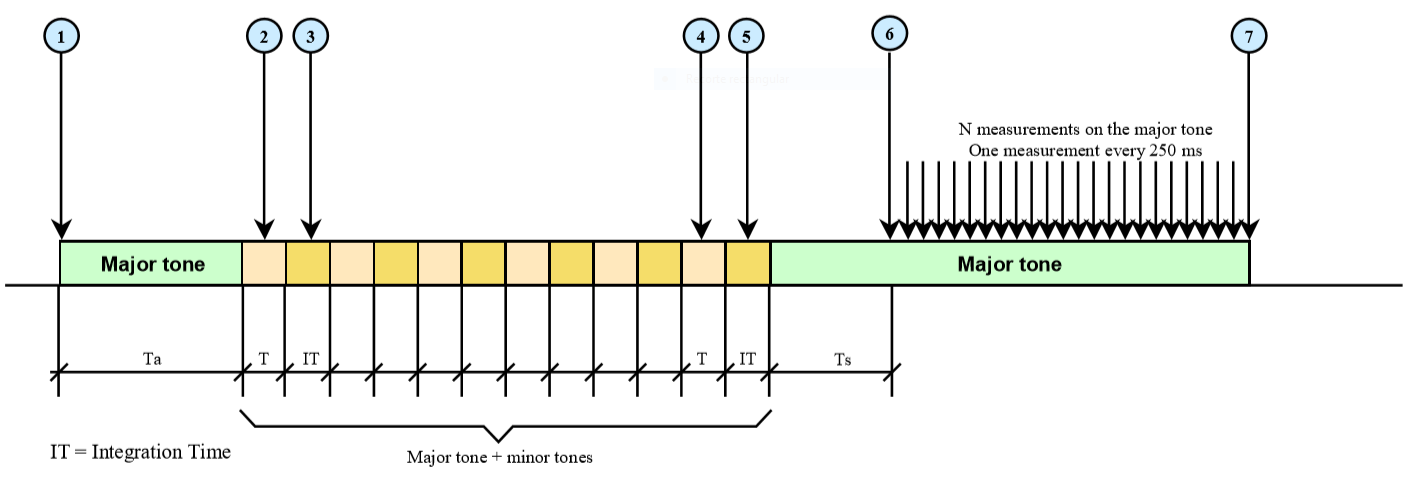
\includegraphics{./diagrams/range_sequence.png}

    \begin{itemize}
\tightlist
\item
  En primer lugar se recibe una petición para medición de rango y se
  genera una señal con el tono mayor por \(T_a\)
\item
  En segundo, se añade un tono menor a la señal de mayor para crear el
  tono virtual necesario por \(T\) segundos
\item
  En tercero, se tomo un tiempo \(IT\) de a lo menos 250ms para la
  medición del desfasamiento del tono virtual
\item
  Se repite este proceso para el resto de los tonos menores
\item
  Despues de lo cual, se queda el tono mayor solamente por \(T_s\)
  segundos
\item
  Y se procede a tomar \(10\) mediciones, una cada \(250ms\)
\end{itemize}

    \begin{tcolorbox}[breakable, size=fbox, boxrule=1pt, pad at break*=1mm,colback=cellbackground, colframe=cellborder]
\prompt{In}{incolor}{4}{\boxspacing}
\begin{Verbatim}[commandchars=\\\{\}]
\PY{n}{ωm} \PY{o}{=} \PY{l+m+mf}{27777.78}
\PY{n}{ωs} \PY{o}{=} \PY{p}{[}\PY{l+m+mf}{22222.22}\PY{p}{,} \PY{l+m+mf}{23333.33}\PY{p}{,} \PY{l+m+mf}{22444.44}\PY{p}{,} \PY{l+m+mf}{22266.67}\PY{p}{,} \PY{l+m+mf}{22231.11}\PY{p}{,} \PY{l+m+mf}{22224.00}\PY{p}{]}
\end{Verbatim}
\end{tcolorbox}

    \begin{tcolorbox}[breakable, size=fbox, boxrule=1pt, pad at break*=1mm,colback=cellbackground, colframe=cellborder]
\prompt{In}{incolor}{5}{\boxspacing}
\begin{Verbatim}[commandchars=\\\{\}]
\PY{n}{Ta} \PY{o}{=} \PY{n}{Ts} \PY{o}{=} \PY{l+m+mi}{2}
\PY{n}{T} \PY{o}{=} \PY{n}{IT} \PY{o}{=} \PY{l+m+mi}{2}

\PY{n}{T0} \PY{o}{=} \PY{l+m+mi}{0}
\PY{n}{Tf} \PY{o}{=} \PY{n}{Ta} \PY{o}{+} \PY{l+m+mi}{6}\PY{o}{*}\PY{p}{(}\PY{n}{T} \PY{o}{+} \PY{n}{IT}\PY{p}{)} \PY{o}{+} \PY{n}{Ts} \PY{o}{+} \PY{l+m+mi}{10}\PY{o}{*}\PY{l+m+mf}{0.25}

\PY{n}{δt} \PY{o}{=} \PY{l+m+mf}{0.000003}
\PY{n}{n} \PY{o}{=} \PY{n+nb}{int}\PY{p}{(}\PY{n}{Tf}\PY{o}{/}\PY{n}{δt}\PY{p}{)} \PY{o}{+} \PY{l+m+mi}{1}

\PY{n}{ts} \PY{o}{=} \PY{n}{linspace}\PY{p}{(}\PY{n}{T0}\PY{p}{,} \PY{n}{Tf}\PY{o}{+}\PY{l+m+mi}{1}\PY{p}{,} \PY{n}{n}\PY{p}{)}

\PY{n}{tm} \PY{o}{=} \PY{n}{linspace}\PY{p}{(}\PY{n}{T0}\PY{p}{,} \PY{n}{Ta} \PY{o}{\PYZhy{}} \PY{n}{δt}\PY{p}{,} \PY{n+nb}{int}\PY{p}{(}\PY{n}{Ta}\PY{o}{/}\PY{n}{δt}\PY{p}{)}\PY{p}{)}
\PY{n}{t1} \PY{o}{=} \PY{n}{linspace}\PY{p}{(}\PY{n}{Ta} \PY{o}{+} \PY{l+m+mi}{0}\PY{o}{*}\PY{p}{(}\PY{n}{T} \PY{o}{+} \PY{n}{IT}\PY{p}{)}\PY{p}{,} \PY{n}{Ta} \PY{o}{+} \PY{l+m+mi}{1}\PY{o}{*}\PY{p}{(}\PY{n}{T} \PY{o}{+} \PY{n}{IT}\PY{p}{)} \PY{o}{\PYZhy{}} \PY{n}{δt}\PY{p}{,} \PY{n+nb}{int}\PY{p}{(}\PY{p}{(}\PY{n}{T} \PY{o}{+} \PY{n}{IT}\PY{p}{)}\PY{o}{/}\PY{n}{δt}\PY{p}{)}\PY{p}{)}
\PY{n}{t2} \PY{o}{=} \PY{n}{linspace}\PY{p}{(}\PY{n}{Ta} \PY{o}{+} \PY{l+m+mi}{1}\PY{o}{*}\PY{p}{(}\PY{n}{T} \PY{o}{+} \PY{n}{IT}\PY{p}{)}\PY{p}{,} \PY{n}{Ta} \PY{o}{+} \PY{l+m+mi}{2}\PY{o}{*}\PY{p}{(}\PY{n}{T} \PY{o}{+} \PY{n}{IT}\PY{p}{)} \PY{o}{\PYZhy{}} \PY{n}{δt}\PY{p}{,} \PY{n+nb}{int}\PY{p}{(}\PY{p}{(}\PY{n}{T} \PY{o}{+} \PY{n}{IT}\PY{p}{)}\PY{o}{/}\PY{n}{δt}\PY{p}{)}\PY{p}{)}
\PY{n}{t3} \PY{o}{=} \PY{n}{linspace}\PY{p}{(}\PY{n}{Ta} \PY{o}{+} \PY{l+m+mi}{2}\PY{o}{*}\PY{p}{(}\PY{n}{T} \PY{o}{+} \PY{n}{IT}\PY{p}{)}\PY{p}{,} \PY{n}{Ta} \PY{o}{+} \PY{l+m+mi}{3}\PY{o}{*}\PY{p}{(}\PY{n}{T} \PY{o}{+} \PY{n}{IT}\PY{p}{)} \PY{o}{\PYZhy{}} \PY{n}{δt}\PY{p}{,} \PY{n+nb}{int}\PY{p}{(}\PY{p}{(}\PY{n}{T} \PY{o}{+} \PY{n}{IT}\PY{p}{)}\PY{o}{/}\PY{n}{δt}\PY{p}{)}\PY{p}{)}
\PY{n}{t4} \PY{o}{=} \PY{n}{linspace}\PY{p}{(}\PY{n}{Ta} \PY{o}{+} \PY{l+m+mi}{3}\PY{o}{*}\PY{p}{(}\PY{n}{T} \PY{o}{+} \PY{n}{IT}\PY{p}{)}\PY{p}{,} \PY{n}{Ta} \PY{o}{+} \PY{l+m+mi}{4}\PY{o}{*}\PY{p}{(}\PY{n}{T} \PY{o}{+} \PY{n}{IT}\PY{p}{)} \PY{o}{\PYZhy{}} \PY{n}{δt}\PY{p}{,} \PY{n+nb}{int}\PY{p}{(}\PY{p}{(}\PY{n}{T} \PY{o}{+} \PY{n}{IT}\PY{p}{)}\PY{o}{/}\PY{n}{δt}\PY{p}{)}\PY{p}{)}
\PY{n}{t5} \PY{o}{=} \PY{n}{linspace}\PY{p}{(}\PY{n}{Ta} \PY{o}{+} \PY{l+m+mi}{4}\PY{o}{*}\PY{p}{(}\PY{n}{T} \PY{o}{+} \PY{n}{IT}\PY{p}{)}\PY{p}{,} \PY{n}{Ta} \PY{o}{+} \PY{l+m+mi}{5}\PY{o}{*}\PY{p}{(}\PY{n}{T} \PY{o}{+} \PY{n}{IT}\PY{p}{)} \PY{o}{\PYZhy{}} \PY{n}{δt}\PY{p}{,} \PY{n+nb}{int}\PY{p}{(}\PY{p}{(}\PY{n}{T} \PY{o}{+} \PY{n}{IT}\PY{p}{)}\PY{o}{/}\PY{n}{δt}\PY{p}{)}\PY{p}{)}
\PY{n}{t6} \PY{o}{=} \PY{n}{linspace}\PY{p}{(}\PY{n}{Ta} \PY{o}{+} \PY{l+m+mi}{5}\PY{o}{*}\PY{p}{(}\PY{n}{T} \PY{o}{+} \PY{n}{IT}\PY{p}{)}\PY{p}{,} \PY{n}{Ta} \PY{o}{+} \PY{l+m+mi}{6}\PY{o}{*}\PY{p}{(}\PY{n}{T} \PY{o}{+} \PY{n}{IT}\PY{p}{)} \PY{o}{\PYZhy{}} \PY{n}{δt}\PY{p}{,} \PY{n+nb}{int}\PY{p}{(}\PY{p}{(}\PY{n}{T} \PY{o}{+} \PY{n}{IT}\PY{p}{)}\PY{o}{/}\PY{n}{δt}\PY{p}{)}\PY{p}{)}
\PY{n}{tw} \PY{o}{=} \PY{n}{linspace}\PY{p}{(}\PY{n}{Ta} \PY{o}{+} \PY{l+m+mi}{6}\PY{o}{*}\PY{p}{(}\PY{n}{T} \PY{o}{+} \PY{n}{IT}\PY{p}{)}\PY{p}{,} \PY{n}{Ta} \PY{o}{+} \PY{l+m+mi}{6}\PY{o}{*}\PY{p}{(}\PY{n}{T} \PY{o}{+} \PY{n}{IT}\PY{p}{)} \PY{o}{+} \PY{n}{Ts} \PY{o}{\PYZhy{}} \PY{n}{δt}\PY{p}{,} \PY{n+nb}{int}\PY{p}{(}\PY{n}{Ts}\PY{o}{/}\PY{n}{δt}\PY{p}{)}\PY{p}{)}
\PY{n}{tmeas} \PY{o}{=} \PY{n}{linspace}\PY{p}{(}\PY{n}{Ta} \PY{o}{+} \PY{l+m+mi}{6}\PY{o}{*}\PY{p}{(}\PY{n}{T} \PY{o}{+} \PY{n}{IT}\PY{p}{)} \PY{o}{+} \PY{n}{Ts}\PY{p}{,} \PY{n}{Tf}\PY{p}{,} \PY{n+nb}{int}\PY{p}{(}\PY{l+m+mi}{10}\PY{o}{*}\PY{l+m+mf}{0.25}\PY{o}{/}\PY{n}{δt}\PY{p}{)}\PY{p}{)}
\PY{n}{tsil} \PY{o}{=} \PY{n}{linspace}\PY{p}{(}\PY{n}{Tf}\PY{p}{,} \PY{n}{Tf} \PY{o}{+} \PY{l+m+mi}{1}\PY{p}{,} \PY{n+nb}{int}\PY{p}{(}\PY{l+m+mi}{1}\PY{o}{/}\PY{n}{δt}\PY{p}{)} \PY{o}{+} \PY{l+m+mi}{1}\PY{p}{)}
\end{Verbatim}
\end{tcolorbox}

    \begin{tcolorbox}[breakable, size=fbox, boxrule=1pt, pad at break*=1mm,colback=cellbackground, colframe=cellborder]
\prompt{In}{incolor}{6}{\boxspacing}
\begin{Verbatim}[commandchars=\\\{\}]
\PY{n}{maj\PYZus{}ton} \PY{o}{=} \PY{k}{lambda} \PY{n}{ts}\PY{p}{:} \PY{n}{sin}\PY{p}{(}\PY{l+m+mi}{2}\PY{o}{*}\PY{n}{pi}\PY{o}{*}\PY{n}{ωm}\PY{o}{*}\PY{n}{ts}\PY{p}{)}
\PY{n}{tone1}   \PY{o}{=} \PY{k}{lambda} \PY{n}{ts}\PY{p}{:} \PY{n}{sin}\PY{p}{(}\PY{l+m+mi}{2}\PY{o}{*}\PY{n}{pi}\PY{o}{*}\PY{n}{ωs}\PY{p}{[}\PY{l+m+mi}{0}\PY{p}{]}\PY{o}{*}\PY{n}{ts}\PY{p}{)}
\PY{n}{tone2}   \PY{o}{=} \PY{k}{lambda} \PY{n}{ts}\PY{p}{:} \PY{n}{sin}\PY{p}{(}\PY{l+m+mi}{2}\PY{o}{*}\PY{n}{pi}\PY{o}{*}\PY{n}{ωs}\PY{p}{[}\PY{l+m+mi}{1}\PY{p}{]}\PY{o}{*}\PY{n}{ts}\PY{p}{)}
\PY{n}{tone3}   \PY{o}{=} \PY{k}{lambda} \PY{n}{ts}\PY{p}{:} \PY{n}{sin}\PY{p}{(}\PY{l+m+mi}{2}\PY{o}{*}\PY{n}{pi}\PY{o}{*}\PY{n}{ωs}\PY{p}{[}\PY{l+m+mi}{2}\PY{p}{]}\PY{o}{*}\PY{n}{ts}\PY{p}{)}
\PY{n}{tone4}   \PY{o}{=} \PY{k}{lambda} \PY{n}{ts}\PY{p}{:} \PY{n}{sin}\PY{p}{(}\PY{l+m+mi}{2}\PY{o}{*}\PY{n}{pi}\PY{o}{*}\PY{n}{ωs}\PY{p}{[}\PY{l+m+mi}{3}\PY{p}{]}\PY{o}{*}\PY{n}{ts}\PY{p}{)}
\PY{n}{tone5}   \PY{o}{=} \PY{k}{lambda} \PY{n}{ts}\PY{p}{:} \PY{n}{sin}\PY{p}{(}\PY{l+m+mi}{2}\PY{o}{*}\PY{n}{pi}\PY{o}{*}\PY{n}{ωs}\PY{p}{[}\PY{l+m+mi}{4}\PY{p}{]}\PY{o}{*}\PY{n}{ts}\PY{p}{)}
\PY{n}{tone6}   \PY{o}{=} \PY{k}{lambda} \PY{n}{ts}\PY{p}{:} \PY{n}{sin}\PY{p}{(}\PY{l+m+mi}{2}\PY{o}{*}\PY{n}{pi}\PY{o}{*}\PY{n}{ωs}\PY{p}{[}\PY{l+m+mi}{5}\PY{p}{]}\PY{o}{*}\PY{n}{ts}\PY{p}{)}

\PY{n}{sm} \PY{o}{=} \PY{n}{maj\PYZus{}ton}\PY{p}{(}\PY{n}{tm}\PY{p}{)}
\PY{n}{s1} \PY{o}{=} \PY{n}{maj\PYZus{}ton}\PY{p}{(}\PY{n}{t1}\PY{p}{)} \PY{o}{+} \PY{n}{tone1}\PY{p}{(}\PY{n}{t1}\PY{p}{)}
\PY{n}{s2} \PY{o}{=} \PY{n}{tone1}\PY{p}{(}\PY{n}{t2}\PY{p}{)} \PY{o}{+} \PY{n}{tone2}\PY{p}{(}\PY{n}{t2}\PY{p}{)}
\PY{n}{s3} \PY{o}{=} \PY{n}{tone1}\PY{p}{(}\PY{n}{t3}\PY{p}{)} \PY{o}{+} \PY{n}{tone3}\PY{p}{(}\PY{n}{t3}\PY{p}{)}
\PY{n}{s4} \PY{o}{=} \PY{n}{tone1}\PY{p}{(}\PY{n}{t4}\PY{p}{)} \PY{o}{+} \PY{n}{tone4}\PY{p}{(}\PY{n}{t4}\PY{p}{)}
\PY{n}{s5} \PY{o}{=} \PY{n}{tone1}\PY{p}{(}\PY{n}{t5}\PY{p}{)} \PY{o}{+} \PY{n}{tone5}\PY{p}{(}\PY{n}{t5}\PY{p}{)}
\PY{n}{s6} \PY{o}{=} \PY{n}{tone1}\PY{p}{(}\PY{n}{t6}\PY{p}{)} \PY{o}{+} \PY{n}{tone6}\PY{p}{(}\PY{n}{t6}\PY{p}{)}
\PY{n}{sw} \PY{o}{=} \PY{n}{maj\PYZus{}ton}\PY{p}{(}\PY{n}{tw}\PY{p}{)}
\PY{n}{smeas} \PY{o}{=} \PY{n}{maj\PYZus{}ton}\PY{p}{(}\PY{n}{tmeas}\PY{p}{)}
\PY{n}{ssil} \PY{o}{=} \PY{n}{array}\PY{p}{(}\PY{p}{[}\PY{l+m+mi}{0} \PY{k}{for} \PY{n}{t} \PY{o+ow}{in} \PY{n}{tsil}\PY{p}{]}\PY{p}{)}
\end{Verbatim}
\end{tcolorbox}

    \begin{tcolorbox}[breakable, size=fbox, boxrule=1pt, pad at break*=1mm,colback=cellbackground, colframe=cellborder]
\prompt{In}{incolor}{7}{\boxspacing}
\begin{Verbatim}[commandchars=\\\{\}]
\PY{k+kn}{from} \PY{n+nn}{matplotlib}\PY{n+nn}{.}\PY{n+nn}{pyplot} \PY{k+kn}{import} \PY{n}{figure}\PY{p}{,} \PY{n}{rcParams}\PY{p}{,} \PY{n}{subplot2grid}
\PY{k+kn}{from} \PY{n+nn}{conf\PYZus{}matplotlib} \PY{k+kn}{import} \PY{n}{conf\PYZus{}matplotlib\PYZus{}claro}
\PY{n}{conf\PYZus{}matplotlib\PYZus{}claro}\PY{p}{(}\PY{p}{)}

\PY{n}{cycle} \PY{o}{=} \PY{n}{rcParams}\PY{p}{[}\PY{l+s+s1}{\PYZsq{}}\PY{l+s+s1}{axes.prop\PYZus{}cycle}\PY{l+s+s1}{\PYZsq{}}\PY{p}{]}\PY{o}{.}\PY{n}{by\PYZus{}key}\PY{p}{(}\PY{p}{)}\PY{p}{[}\PY{l+s+s1}{\PYZsq{}}\PY{l+s+s1}{color}\PY{l+s+s1}{\PYZsq{}}\PY{p}{]}
\PY{n}{colores} \PY{o}{=} \PY{p}{[}\PY{n+nb}{tuple}\PY{p}{(}\PY{n+nb}{int}\PY{p}{(}\PY{n}{h}\PY{o}{.}\PY{n}{lstrip}\PY{p}{(}\PY{l+s+s1}{\PYZsq{}}\PY{l+s+s1}{\PYZsh{}}\PY{l+s+s1}{\PYZsq{}}\PY{p}{)}\PY{p}{[}\PY{n}{i}\PY{p}{:}\PY{n}{i}\PY{o}{+}\PY{l+m+mi}{2}\PY{p}{]}\PY{p}{,} \PY{l+m+mi}{16}\PY{p}{)} \PY{k}{for} \PY{n}{i} \PY{o+ow}{in} \PY{p}{(}\PY{l+m+mi}{0}\PY{p}{,} \PY{l+m+mi}{2}\PY{p}{,} \PY{l+m+mi}{4}\PY{p}{)}\PY{p}{)} \PY{k}{for} \PY{n}{h} \PY{o+ow}{in} \PY{n}{cycle}\PY{p}{]}
\end{Verbatim}
\end{tcolorbox}

    Estos tonos son enviados de acuerdo a la secuencia de la figura
anterior, primero el major tone, despues los minor tones en combinación,
seguido de un periodo para la estabilización del PLL y por ultimo las
\(10\) mediciones de rango que vemos en archivos y event viewer con el
major tone solamente.

    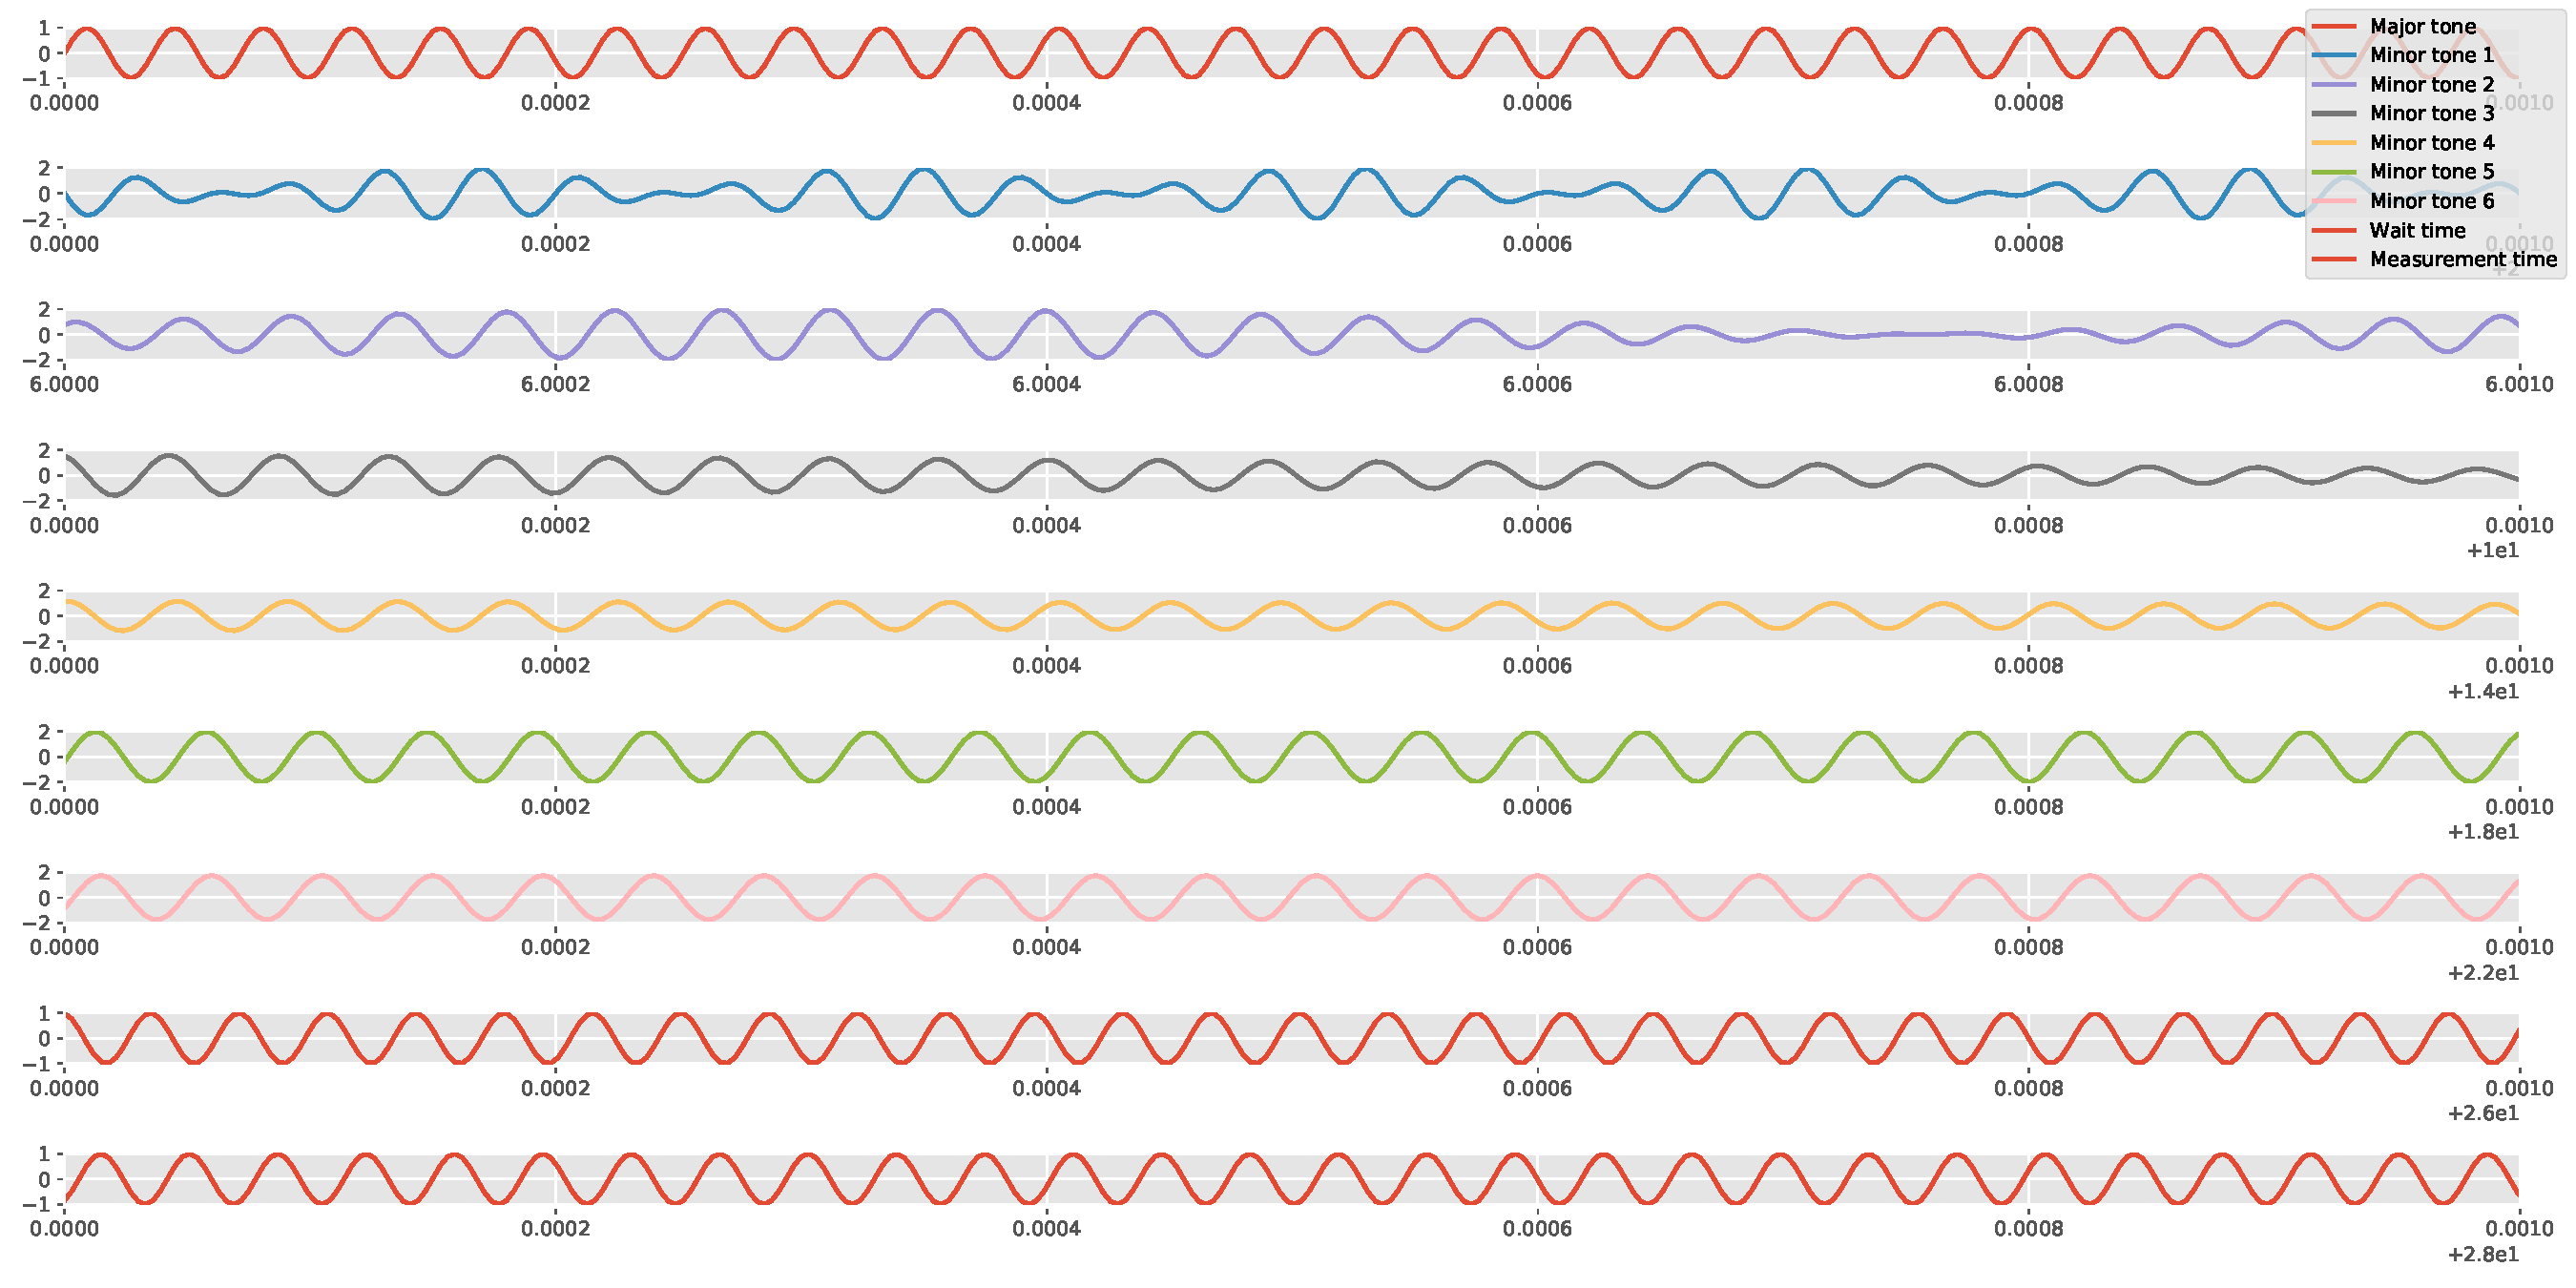
\includegraphics{./muestras-sec-rango.pdf}

    \begin{tcolorbox}[breakable, size=fbox, boxrule=1pt, pad at break*=1mm,colback=cellbackground, colframe=cellborder]
\prompt{In}{incolor}{9}{\boxspacing}
\begin{Verbatim}[commandchars=\\\{\}]
\PY{n}{ts} \PY{o}{=} \PY{n}{concatenate}\PY{p}{(}\PY{p}{[}\PY{n}{tm}\PY{p}{,} \PY{n}{t1}\PY{p}{,} \PY{n}{t2}\PY{p}{,} \PY{n}{t3}\PY{p}{,} \PY{n}{t4}\PY{p}{,} \PY{n}{t5}\PY{p}{,} \PY{n}{t6}\PY{p}{,} \PY{n}{tw}\PY{p}{,} \PY{n}{tmeas}\PY{p}{,} \PY{n}{tsil}\PY{p}{]}\PY{p}{)}
\PY{n}{ss} \PY{o}{=} \PY{n}{concatenate}\PY{p}{(}\PY{p}{[}\PY{n}{sm}\PY{p}{,} \PY{n}{s1}\PY{p}{,} \PY{n}{s2}\PY{p}{,} \PY{n}{s3}\PY{p}{,} \PY{n}{s4}\PY{p}{,} \PY{n}{s5}\PY{p}{,} \PY{n}{s6}\PY{p}{,} \PY{n}{sw}\PY{p}{,} \PY{n}{smeas}\PY{p}{,} \PY{n}{ssil}\PY{p}{]}\PY{p}{)}
\end{Verbatim}
\end{tcolorbox}

    \hypertarget{efectos-internos}{%
\subsection{Efectos internos}\label{efectos-internos}}

    Existen factores que estan involucrados con el tiempo medido por el
sistema de rango, es facil dividirlos como internos y externos.

    \begin{itemize}
\tightlist
\item
  Retraso en equipo de tierra
\end{itemize}

    Un factor interno es el retraso en el equipo de tierra, el cual esta
considerado en los archivos de calibración, por lo que es importante
tener en cuenta que este debe coincidir con la cadena de RF utilizada
actualmente.

    \begin{itemize}
\tightlist
\item
  Amplificación en nave
\end{itemize}

    El retardo en el equipo de retransmisión de la nave es siempre el mismo,
siempre y cuando la configuración de enrutamiento de rango sea el
adecuado. Si se configura la transmisión de comandos y rango por la
frecuencia asociada al CMR2, es necesario que tambien se configure la
ruta para la señal de rango del CMR2 al TTX1 en caso de tener el
transmisor de telemetria 1.

    \hypertarget{efectos-externos}{%
\subsection{Efectos externos}\label{efectos-externos}}

    \begin{itemize}
\tightlist
\item
  Distancia del centro de control al satelite
\end{itemize}

    La distancia del centro de control al satelite es variable y es
justamente el parametro a medir para una adecuada determinación de
orbita. Para la simulación actual se utiliza el valor
\(\rho = 36,480.152km\).

    \begin{tcolorbox}[breakable, size=fbox, boxrule=1pt, pad at break*=1mm,colback=cellbackground, colframe=cellborder]
\prompt{In}{incolor}{10}{\boxspacing}
\begin{Verbatim}[commandchars=\\\{\}]
\PY{k+kn}{from} \PY{n+nn}{scipy}\PY{n+nn}{.}\PY{n+nn}{constants} \PY{k+kn}{import} \PY{n}{c}

\PY{n}{distancia\PYZus{}ant\PYZus{}sat} \PY{o}{=} \PY{l+m+mf}{36.480152e6}
\PY{n}{delay} \PY{o}{=} \PY{l+m+mi}{2}\PY{o}{*}\PY{n}{distancia\PYZus{}ant\PYZus{}sat}\PY{o}{/}\PY{n}{c}
\PY{n}{delay}
\end{Verbatim}
\end{tcolorbox}

            \begin{tcolorbox}[breakable, size=fbox, boxrule=.5pt, pad at break*=1mm, opacityfill=0]
\prompt{Out}{outcolor}{10}{\boxspacing}
\begin{Verbatim}[commandchars=\\\{\}]
0.24336937789142113
\end{Verbatim}
\end{tcolorbox}

    \begin{itemize}
\tightlist
\item
  Efectos de atenuación por fenomenos atmosféricos
\end{itemize}

    \begin{tcolorbox}[breakable, size=fbox, boxrule=1pt, pad at break*=1mm,colback=cellbackground, colframe=cellborder]
\prompt{In}{incolor}{11}{\boxspacing}
\begin{Verbatim}[commandchars=\\\{\}]
\PY{n}{top} \PY{o}{=} \PY{n}{concatenate}\PY{p}{(}\PY{p}{[}\PY{n}{array}\PY{p}{(}\PY{p}{[}\PY{l+m+mi}{0}\PY{p}{,} \PY{n}{ts}\PY{p}{[}\PY{l+m+mi}{0}\PY{p}{]} \PY{o}{\PYZhy{}} \PY{n}{δt}\PY{p}{]}\PY{p}{)}\PY{p}{,} \PY{n}{array}\PY{p}{(}\PY{p}{[}\PY{n}{t} \PY{o}{+} \PY{n}{delay} \PY{k}{for} \PY{n}{t} \PY{o+ow}{in} \PY{n}{ts}\PY{p}{]}\PY{p}{)}\PY{p}{]}\PY{p}{)}
\PY{n}{sop} \PY{o}{=} \PY{n}{concatenate}\PY{p}{(}\PY{p}{[}\PY{n}{array}\PY{p}{(}\PY{p}{[}\PY{l+m+mi}{0}\PY{p}{,} \PY{l+m+mi}{0}\PY{p}{]}\PY{p}{)}\PY{p}{,} \PY{n}{ss}\PY{p}{]}\PY{p}{)}

\PY{n}{to} \PY{o}{=} \PY{n}{ts}
\PY{n}{so} \PY{o}{=} \PY{n}{array}\PY{p}{(}\PY{p}{[}\PY{n}{interp}\PY{p}{(}\PY{n}{t}\PY{p}{,} \PY{n}{top}\PY{p}{,} \PY{n}{sop}\PY{p}{)} \PY{k}{for} \PY{n}{t} \PY{o+ow}{in} \PY{n}{to}\PY{p}{]}\PY{p}{)}
\end{Verbatim}
\end{tcolorbox}

    Los efectos de atenuación por fenomenos atmosféricos (clima) no son
considerados dentro de esta simulación debido a que tomaria demasiado
tiempo hacer un algoritmo robusto para enfrentar estos efectos, sin
embargo se puede comentar que estos efectos son compensados en menor
medida por la amplificación de la señal repetida por la nave, y en mayor
medida por el PLL interno al cortex de la BBU en tierra.

    \hypertarget{tonos-virtuales}{%
\subsection{Tonos virtuales}\label{tonos-virtuales}}

    \begin{tcolorbox}[breakable, size=fbox, boxrule=1pt, pad at break*=1mm,colback=cellbackground, colframe=cellborder]
\prompt{In}{incolor}{12}{\boxspacing}
\begin{Verbatim}[commandchars=\\\{\}]
\PY{n}{hss} \PY{o}{=} \PY{n+nb}{abs}\PY{p}{(}\PY{n}{hilbert}\PY{p}{(}\PY{n}{ss}\PY{p}{)}\PY{p}{)}
\PY{n}{hso} \PY{o}{=} \PY{n+nb}{abs}\PY{p}{(}\PY{n}{hilbert}\PY{p}{(}\PY{n}{so}\PY{p}{)}\PY{p}{)}
\end{Verbatim}
\end{tcolorbox}

    \begin{tcolorbox}[breakable, size=fbox, boxrule=1pt, pad at break*=1mm,colback=cellbackground, colframe=cellborder]
\prompt{In}{incolor}{13}{\boxspacing}
\begin{Verbatim}[commandchars=\\\{\}]
\PY{n}{ωsv} \PY{o}{=} \PY{p}{[}\PY{l+m+mf}{5555.56}\PY{p}{,} \PY{l+m+mf}{1111.11}\PY{p}{,} \PY{l+m+mf}{222.22}\PY{p}{,} \PY{l+m+mf}{44.44}\PY{p}{,} \PY{l+m+mf}{8.89}\PY{p}{,} \PY{l+m+mf}{1.78}\PY{p}{]}
\end{Verbatim}
\end{tcolorbox}

    \begin{tcolorbox}[breakable, size=fbox, boxrule=1pt, pad at break*=1mm,colback=cellbackground, colframe=cellborder]
\prompt{In}{incolor}{14}{\boxspacing}
\begin{Verbatim}[commandchars=\\\{\}]
\PY{k}{def} \PY{n+nf}{tono1\PYZus{}virtual}\PY{p}{(}\PY{n}{α} \PY{o}{=} \PY{l+m+mi}{1}\PY{p}{)}\PY{p}{:}
    \PY{n}{fig} \PY{o}{=} \PY{n}{figure}\PY{p}{(}\PY{n}{figsize}\PY{o}{=}\PY{p}{(}\PY{l+m+mi}{18}\PY{p}{,}\PY{l+m+mi}{4}\PY{p}{)}\PY{p}{)}
    \PY{n}{ax} \PY{o}{=} \PY{n}{fig}\PY{o}{.}\PY{n}{gca}\PY{p}{(}\PY{p}{)}
    \PY{n}{ax}\PY{o}{.}\PY{n}{plot}\PY{p}{(}\PY{n}{ts}\PY{p}{,} \PY{n}{ss}\PY{p}{,} \PY{n}{lw}\PY{o}{=}\PY{l+m+mi}{2}\PY{p}{,} \PY{n}{c}\PY{o}{=}\PY{n}{cycle}\PY{p}{[}\PY{l+m+mi}{0}\PY{p}{]}\PY{p}{,} \PY{n}{alpha}\PY{o}{=}\PY{n}{α}\PY{p}{)}
    \PY{n}{ax}\PY{o}{.}\PY{n}{plot}\PY{p}{(}\PY{n}{ts}\PY{p}{,} \PY{n}{hss}\PY{p}{,} \PY{l+s+s2}{\PYZdq{}}\PY{l+s+s2}{\PYZhy{}\PYZhy{}}\PY{l+s+s2}{\PYZdq{}}\PY{p}{,} \PY{n}{lw}\PY{o}{=}\PY{l+m+mi}{2}\PY{p}{,} \PY{n}{c}\PY{o}{=}\PY{n}{cycle}\PY{p}{[}\PY{l+m+mi}{0}\PY{p}{]}\PY{p}{,} \PY{n}{alpha}\PY{o}{=}\PY{l+m+mi}{1}\PY{o}{\PYZhy{}}\PY{n}{α}\PY{p}{)}
    \PY{n}{ax}\PY{o}{.}\PY{n}{plot}\PY{p}{(}\PY{n}{to}\PY{p}{,} \PY{n}{so}\PY{p}{,} \PY{n}{lw}\PY{o}{=}\PY{l+m+mi}{2}\PY{p}{,} \PY{n}{c}\PY{o}{=}\PY{n}{cycle}\PY{p}{[}\PY{l+m+mi}{1}\PY{p}{]}\PY{p}{,} \PY{n}{alpha}\PY{o}{=}\PY{n}{α}\PY{p}{)}
    \PY{n}{ax}\PY{o}{.}\PY{n}{plot}\PY{p}{(}\PY{n}{to}\PY{p}{,} \PY{n}{hso}\PY{p}{,} \PY{l+s+s2}{\PYZdq{}}\PY{l+s+s2}{\PYZhy{}\PYZhy{}}\PY{l+s+s2}{\PYZdq{}}\PY{p}{,} \PY{n}{lw}\PY{o}{=}\PY{l+m+mi}{2}\PY{p}{,} \PY{n}{c}\PY{o}{=}\PY{n}{cycle}\PY{p}{[}\PY{l+m+mi}{1}\PY{p}{]}\PY{p}{,} \PY{n}{alpha}\PY{o}{=}\PY{l+m+mi}{1}\PY{o}{\PYZhy{}}\PY{n}{α}\PY{p}{)}
    \PY{n}{ax}\PY{o}{.}\PY{n}{set\PYZus{}xlim}\PY{p}{(}\PY{n}{t1}\PY{p}{[}\PY{l+m+mi}{0}\PY{p}{]} \PY{o}{+} \PY{l+m+mf}{0.25}\PY{p}{,} \PY{n}{t1}\PY{p}{[}\PY{l+m+mi}{0}\PY{p}{]} \PY{o}{+} \PY{l+m+mf}{0.25} \PY{o}{+} \PY{l+m+mi}{2}\PY{o}{/}\PY{n}{ωsv}\PY{p}{[}\PY{l+m+mi}{0}\PY{p}{]}\PY{p}{)}\PY{p}{;}
\end{Verbatim}
\end{tcolorbox}

    \begin{tcolorbox}[breakable, size=fbox, boxrule=1pt, pad at break*=1mm,colback=cellbackground, colframe=cellborder]
\prompt{In}{incolor}{36}{\boxspacing}
\begin{Verbatim}[commandchars=\\\{\}]
\PY{n}{tono1\PYZus{}virtual}\PY{p}{(}\PY{n}{α}\PY{o}{=}\PY{l+m+mf}{0.4}\PY{p}{)}
\end{Verbatim}
\end{tcolorbox}

    \begin{center}
    \adjustimage{max size={0.9\linewidth}{0.9\paperheight}}{output_33_0.png}
    \end{center}
    { \hspace*{\fill} \\}

    La transmisión de los minor tones anteriores a las mediciones de rango,
se hacen en conjunto, de tal manera que se crea interferencia
constructiva y destructiva (modulación), en la señal final de los minor
tones y se cree un tono virtual, equivalente a la diferencia de las
frecuencias de los minor tones.

    \begin{tcolorbox}[breakable, size=fbox, boxrule=1pt, pad at break*=1mm,colback=cellbackground, colframe=cellborder]
\prompt{In}{incolor}{16}{\boxspacing}
\begin{Verbatim}[commandchars=\\\{\}]
\PY{n}{ωsv} \PY{o}{=} \PY{p}{[}\PY{l+m+mf}{5555.56}\PY{p}{,} \PY{l+m+mf}{1111.11}\PY{p}{,} \PY{l+m+mf}{222.22}\PY{p}{,} \PY{l+m+mf}{44.44}\PY{p}{,} \PY{l+m+mf}{8.89}\PY{p}{,} \PY{l+m+mf}{1.78}\PY{p}{]}
\end{Verbatim}
\end{tcolorbox}

    \begin{tcolorbox}[breakable, size=fbox, boxrule=1pt, pad at break*=1mm,colback=cellbackground, colframe=cellborder]
\prompt{In}{incolor}{17}{\boxspacing}
\begin{Verbatim}[commandchars=\\\{\}]
\PY{k}{def} \PY{n+nf}{grafica\PYZus{}liss\PYZus{}sen}\PY{p}{(}\PY{n}{periodo}\PY{o}{=}\PY{l+s+s2}{\PYZdq{}}\PY{l+s+s2}{Minor tone 1}\PY{l+s+s2}{\PYZdq{}}\PY{p}{)}\PY{p}{:}
    \PY{k+kn}{from} \PY{n+nn}{numpy} \PY{k+kn}{import} \PY{n}{arcsin}\PY{p}{,} \PY{n}{degrees}

    \PY{n}{options} \PY{o}{=} \PY{p}{\PYZob{}}\PY{l+s+s2}{\PYZdq{}}\PY{l+s+s2}{Major tone}\PY{l+s+s2}{\PYZdq{}}\PY{p}{:} \PY{n}{tm}\PY{p}{,}
               \PY{l+s+s2}{\PYZdq{}}\PY{l+s+s2}{Minor tone 1}\PY{l+s+s2}{\PYZdq{}}\PY{p}{:} \PY{n}{t1}\PY{p}{,}
               \PY{l+s+s2}{\PYZdq{}}\PY{l+s+s2}{Minor tone 2}\PY{l+s+s2}{\PYZdq{}}\PY{p}{:} \PY{n}{t2}\PY{p}{,}
               \PY{l+s+s2}{\PYZdq{}}\PY{l+s+s2}{Minor tone 3}\PY{l+s+s2}{\PYZdq{}}\PY{p}{:} \PY{n}{t3}\PY{p}{,}
               \PY{l+s+s2}{\PYZdq{}}\PY{l+s+s2}{Minor tone 4}\PY{l+s+s2}{\PYZdq{}}\PY{p}{:} \PY{n}{t4}\PY{p}{,}
               \PY{l+s+s2}{\PYZdq{}}\PY{l+s+s2}{Minor tone 5}\PY{l+s+s2}{\PYZdq{}}\PY{p}{:} \PY{n}{t5}\PY{p}{,}
               \PY{l+s+s2}{\PYZdq{}}\PY{l+s+s2}{Minor tone 6}\PY{l+s+s2}{\PYZdq{}}\PY{p}{:} \PY{n}{t6}\PY{p}{,}
               \PY{l+s+s2}{\PYZdq{}}\PY{l+s+s2}{Waiting time}\PY{l+s+s2}{\PYZdq{}}\PY{p}{:} \PY{n}{tw}\PY{p}{,}
               \PY{l+s+s2}{\PYZdq{}}\PY{l+s+s2}{Measurement time}\PY{l+s+s2}{\PYZdq{}}\PY{p}{:} \PY{n}{tmeas}\PY{p}{\PYZcb{}}

    \PY{n}{tspans}  \PY{o}{=} \PY{p}{\PYZob{}}\PY{l+s+s2}{\PYZdq{}}\PY{l+s+s2}{Major tone}\PY{l+s+s2}{\PYZdq{}}\PY{p}{:} \PY{l+m+mf}{1.2}\PY{o}{/}\PY{n}{ωm}\PY{p}{,}
               \PY{l+s+s2}{\PYZdq{}}\PY{l+s+s2}{Minor tone 1}\PY{l+s+s2}{\PYZdq{}}\PY{p}{:} \PY{l+m+mf}{1.2}\PY{o}{/}\PY{n}{ωsv}\PY{p}{[}\PY{l+m+mi}{0}\PY{p}{]}\PY{p}{,}
               \PY{l+s+s2}{\PYZdq{}}\PY{l+s+s2}{Minor tone 2}\PY{l+s+s2}{\PYZdq{}}\PY{p}{:} \PY{l+m+mf}{1.2}\PY{o}{/}\PY{n}{ωsv}\PY{p}{[}\PY{l+m+mi}{1}\PY{p}{]}\PY{p}{,}
               \PY{l+s+s2}{\PYZdq{}}\PY{l+s+s2}{Minor tone 3}\PY{l+s+s2}{\PYZdq{}}\PY{p}{:} \PY{l+m+mf}{1.2}\PY{o}{/}\PY{n}{ωsv}\PY{p}{[}\PY{l+m+mi}{2}\PY{p}{]}\PY{p}{,}
               \PY{l+s+s2}{\PYZdq{}}\PY{l+s+s2}{Minor tone 4}\PY{l+s+s2}{\PYZdq{}}\PY{p}{:} \PY{l+m+mf}{1.2}\PY{o}{/}\PY{n}{ωsv}\PY{p}{[}\PY{l+m+mi}{3}\PY{p}{]}\PY{p}{,}
               \PY{l+s+s2}{\PYZdq{}}\PY{l+s+s2}{Minor tone 5}\PY{l+s+s2}{\PYZdq{}}\PY{p}{:} \PY{l+m+mf}{1.2}\PY{o}{/}\PY{n}{ωsv}\PY{p}{[}\PY{l+m+mi}{4}\PY{p}{]}\PY{p}{,}
               \PY{l+s+s2}{\PYZdq{}}\PY{l+s+s2}{Minor tone 6}\PY{l+s+s2}{\PYZdq{}}\PY{p}{:} \PY{l+m+mf}{1.2}\PY{o}{/}\PY{n}{ωsv}\PY{p}{[}\PY{l+m+mi}{5}\PY{p}{]}\PY{p}{,}
               \PY{l+s+s2}{\PYZdq{}}\PY{l+s+s2}{Waiting time}\PY{l+s+s2}{\PYZdq{}}\PY{p}{:} \PY{l+m+mf}{1.2}\PY{o}{/}\PY{n}{ωm}\PY{p}{,}
               \PY{l+s+s2}{\PYZdq{}}\PY{l+s+s2}{Measurement time}\PY{l+s+s2}{\PYZdq{}}\PY{p}{:} \PY{l+m+mf}{1.2}\PY{o}{/}\PY{n}{ωm}\PY{p}{\PYZcb{}}

    \PY{n}{per} \PY{o}{=} \PY{n}{options}\PY{p}{[}\PY{n}{periodo}\PY{p}{]}
    \PY{n}{Δt} \PY{o}{=} \PY{n}{tspans}\PY{p}{[}\PY{n}{periodo}\PY{p}{]}

    \PY{n}{t0} \PY{o}{=} \PY{n}{per}\PY{p}{[}\PY{l+m+mi}{0}\PY{p}{]} \PY{o}{+} \PY{l+m+mf}{0.25}
    \PY{n}{tf} \PY{o}{=} \PY{n}{t0} \PY{o}{+} \PY{n}{Δt}
    \PY{n}{ind\PYZus{}ini} \PY{o}{=} \PY{n}{where}\PY{p}{(}\PY{n}{ts} \PY{o}{\PYZlt{}}\PY{o}{=} \PY{n}{t0}\PY{p}{)}\PY{p}{[}\PY{l+m+mi}{0}\PY{p}{]}\PY{p}{[}\PY{o}{\PYZhy{}}\PY{l+m+mi}{1}\PY{p}{]}
    \PY{n}{ind\PYZus{}fin} \PY{o}{=} \PY{n}{where}\PY{p}{(}\PY{n}{ts} \PY{o}{\PYZlt{}}\PY{o}{=} \PY{n}{tf}\PY{p}{)}\PY{p}{[}\PY{l+m+mi}{0}\PY{p}{]}\PY{p}{[}\PY{o}{\PYZhy{}}\PY{l+m+mi}{1}\PY{p}{]}

    \PY{n}{fig} \PY{o}{=} \PY{n}{figure}\PY{p}{(}\PY{n}{figsize}\PY{o}{=}\PY{p}{(}\PY{l+m+mi}{20}\PY{p}{,} \PY{l+m+mi}{5}\PY{p}{)}\PY{p}{)}
    \PY{n}{ax1} \PY{o}{=} \PY{n}{subplot2grid}\PY{p}{(}\PY{p}{(}\PY{l+m+mi}{1}\PY{p}{,}\PY{l+m+mi}{4}\PY{p}{)}\PY{p}{,} \PY{p}{(}\PY{l+m+mi}{0}\PY{p}{,}\PY{l+m+mi}{0}\PY{p}{)}\PY{p}{)}
    \PY{n}{ax2} \PY{o}{=} \PY{n}{subplot2grid}\PY{p}{(}\PY{p}{(}\PY{l+m+mi}{1}\PY{p}{,}\PY{l+m+mi}{4}\PY{p}{)}\PY{p}{,} \PY{p}{(}\PY{l+m+mi}{0}\PY{p}{,}\PY{l+m+mi}{1}\PY{p}{)}\PY{p}{,} \PY{n}{colspan}\PY{o}{=}\PY{l+m+mi}{3}\PY{p}{)}

    \PY{k}{if} \PY{n}{periodo}\PY{p}{[}\PY{l+m+mi}{0}\PY{p}{:}\PY{l+m+mi}{5}\PY{p}{]} \PY{o}{==} \PY{l+s+s2}{\PYZdq{}}\PY{l+s+s2}{Minor}\PY{l+s+s2}{\PYZdq{}}\PY{p}{:}
        \PY{n}{ind\PYZus{}cur1} \PY{o}{=} \PY{n}{where}\PY{p}{(}\PY{n}{hss} \PY{o}{==} \PY{n+nb}{max}\PY{p}{(}\PY{n}{hss}\PY{p}{[}\PY{n}{ind\PYZus{}ini}\PY{p}{:}\PY{n}{ind\PYZus{}fin}\PY{p}{]}\PY{p}{)}\PY{p}{)}\PY{p}{[}\PY{l+m+mi}{0}\PY{p}{]}\PY{p}{[}\PY{l+m+mi}{0}\PY{p}{]}
        \PY{n}{ind\PYZus{}cur2} \PY{o}{=} \PY{n}{where}\PY{p}{(}\PY{n}{hso} \PY{o}{==} \PY{n+nb}{max}\PY{p}{(}\PY{n}{hso}\PY{p}{[}\PY{n}{ind\PYZus{}ini}\PY{p}{:}\PY{n}{ind\PYZus{}fin}\PY{p}{]}\PY{p}{)}\PY{p}{)}\PY{p}{[}\PY{l+m+mi}{0}\PY{p}{]}\PY{p}{[}\PY{l+m+mi}{0}\PY{p}{]}
        \PY{n}{t\PYZus{}cur1} \PY{o}{=} \PY{n}{ts}\PY{p}{[}\PY{n}{ind\PYZus{}cur1}\PY{p}{]}
        \PY{n}{t\PYZus{}cur2} \PY{o}{=} \PY{n}{ts}\PY{p}{[}\PY{n}{ind\PYZus{}cur2}\PY{p}{]}

        \PY{n}{ax1}\PY{o}{.}\PY{n}{plot}\PY{p}{(}\PY{n}{hss}\PY{p}{[}\PY{n}{ind\PYZus{}ini}\PY{p}{:}\PY{n}{ind\PYZus{}fin}\PY{p}{]}\PY{p}{,} \PY{n}{hso}\PY{p}{[}\PY{n}{ind\PYZus{}ini}\PY{p}{:}\PY{n}{ind\PYZus{}fin}\PY{p}{]}\PY{p}{,} \PY{n}{lw}\PY{o}{=}\PY{l+m+mi}{2}\PY{p}{,} \PY{n}{c}\PY{o}{=}\PY{n}{cycle}\PY{p}{[}\PY{l+m+mi}{3}\PY{p}{]}\PY{p}{)}
        \PY{n}{ax1}\PY{o}{.}\PY{n}{plot}\PY{p}{(}\PY{n}{hss}\PY{p}{[}\PY{n}{ind\PYZus{}cur1}\PY{p}{]}\PY{p}{,} \PY{n}{hso}\PY{p}{[}\PY{n}{ind\PYZus{}cur1}\PY{p}{]}\PY{p}{,} \PY{l+s+s2}{\PYZdq{}}\PY{l+s+s2}{o}\PY{l+s+s2}{\PYZdq{}}\PY{p}{,} \PY{n}{c}\PY{o}{=}\PY{n}{cycle}\PY{p}{[}\PY{l+m+mi}{2}\PY{p}{]}\PY{p}{)}
        \PY{n}{ax1}\PY{o}{.}\PY{n}{plot}\PY{p}{(}\PY{n}{hss}\PY{p}{[}\PY{n}{ind\PYZus{}cur2}\PY{p}{]}\PY{p}{,} \PY{n}{hso}\PY{p}{[}\PY{n}{ind\PYZus{}cur2}\PY{p}{]}\PY{p}{,} \PY{l+s+s2}{\PYZdq{}}\PY{l+s+s2}{o}\PY{l+s+s2}{\PYZdq{}}\PY{p}{,} \PY{n}{c}\PY{o}{=}\PY{n}{cycle}\PY{p}{[}\PY{l+m+mi}{4}\PY{p}{]}\PY{p}{)}

        \PY{n}{ax2}\PY{o}{.}\PY{n}{plot}\PY{p}{(}\PY{n}{ts}\PY{p}{,} \PY{n}{ss}\PY{p}{,} \PY{n}{lw}\PY{o}{=}\PY{l+m+mi}{2}\PY{p}{,} \PY{n}{c}\PY{o}{=}\PY{n}{cycle}\PY{p}{[}\PY{l+m+mi}{0}\PY{p}{]}\PY{p}{,} \PY{n}{alpha}\PY{o}{=}\PY{l+m+mf}{0.3}\PY{p}{)}
        \PY{n}{ax2}\PY{o}{.}\PY{n}{plot}\PY{p}{(}\PY{n}{ts}\PY{p}{,} \PY{n}{hss}\PY{p}{,} \PY{l+s+s2}{\PYZdq{}}\PY{l+s+s2}{\PYZhy{}\PYZhy{}}\PY{l+s+s2}{\PYZdq{}}\PY{p}{,} \PY{n}{lw}\PY{o}{=}\PY{l+m+mi}{2}\PY{p}{,} \PY{n}{c}\PY{o}{=}\PY{n}{cycle}\PY{p}{[}\PY{l+m+mi}{0}\PY{p}{]}\PY{p}{)}
        \PY{n}{ax2}\PY{o}{.}\PY{n}{plot}\PY{p}{(}\PY{n}{to}\PY{p}{,} \PY{n}{so}\PY{p}{,} \PY{n}{lw}\PY{o}{=}\PY{l+m+mi}{2}\PY{p}{,} \PY{n}{c}\PY{o}{=}\PY{n}{cycle}\PY{p}{[}\PY{l+m+mi}{1}\PY{p}{]}\PY{p}{,} \PY{n}{alpha}\PY{o}{=}\PY{l+m+mf}{0.3}\PY{p}{)}
        \PY{n}{ax2}\PY{o}{.}\PY{n}{plot}\PY{p}{(}\PY{n}{to}\PY{p}{,} \PY{n}{hso}\PY{p}{,} \PY{l+s+s2}{\PYZdq{}}\PY{l+s+s2}{\PYZhy{}\PYZhy{}}\PY{l+s+s2}{\PYZdq{}}\PY{p}{,} \PY{n}{lw}\PY{o}{=}\PY{l+m+mi}{2}\PY{p}{,} \PY{n}{c}\PY{o}{=}\PY{n}{cycle}\PY{p}{[}\PY{l+m+mi}{1}\PY{p}{]}\PY{p}{)}
    \PY{k}{else}\PY{p}{:}
        \PY{n}{ind\PYZus{}cur1} \PY{o}{=} \PY{n}{where}\PY{p}{(}\PY{n}{ss} \PY{o}{==} \PY{n+nb}{max}\PY{p}{(}\PY{n}{ss}\PY{p}{[}\PY{n}{ind\PYZus{}ini}\PY{p}{:}\PY{n}{ind\PYZus{}fin}\PY{p}{]}\PY{p}{)}\PY{p}{)}\PY{p}{[}\PY{l+m+mi}{0}\PY{p}{]}\PY{p}{[}\PY{l+m+mi}{0}\PY{p}{]}
        \PY{n}{ind\PYZus{}cur2} \PY{o}{=} \PY{n}{where}\PY{p}{(}\PY{n}{so} \PY{o}{==} \PY{n+nb}{max}\PY{p}{(}\PY{n}{so}\PY{p}{[}\PY{n}{ind\PYZus{}ini}\PY{p}{:}\PY{n}{ind\PYZus{}fin}\PY{p}{]}\PY{p}{)}\PY{p}{)}\PY{p}{[}\PY{l+m+mi}{0}\PY{p}{]}\PY{p}{[}\PY{l+m+mi}{0}\PY{p}{]}
        \PY{n}{t\PYZus{}cur1} \PY{o}{=} \PY{n}{ts}\PY{p}{[}\PY{n}{ind\PYZus{}cur1}\PY{p}{]}
        \PY{n}{t\PYZus{}cur2} \PY{o}{=} \PY{n}{ts}\PY{p}{[}\PY{n}{ind\PYZus{}cur2}\PY{p}{]}

        \PY{n}{ax1}\PY{o}{.}\PY{n}{plot}\PY{p}{(}\PY{n}{ss}\PY{p}{[}\PY{n}{ind\PYZus{}ini}\PY{p}{:}\PY{n}{ind\PYZus{}fin}\PY{p}{]}\PY{p}{,} \PY{n}{so}\PY{p}{[}\PY{n}{ind\PYZus{}ini}\PY{p}{:}\PY{n}{ind\PYZus{}fin}\PY{p}{]}\PY{p}{,} \PY{n}{lw}\PY{o}{=}\PY{l+m+mi}{2}\PY{p}{,} \PY{n}{c}\PY{o}{=}\PY{n}{cycle}\PY{p}{[}\PY{l+m+mi}{3}\PY{p}{]}\PY{p}{)}
        \PY{n}{ax1}\PY{o}{.}\PY{n}{plot}\PY{p}{(}\PY{n}{ss}\PY{p}{[}\PY{n}{ind\PYZus{}cur1}\PY{p}{]}\PY{p}{,} \PY{n}{so}\PY{p}{[}\PY{n}{ind\PYZus{}cur1}\PY{p}{]}\PY{p}{,} \PY{l+s+s2}{\PYZdq{}}\PY{l+s+s2}{o}\PY{l+s+s2}{\PYZdq{}}\PY{p}{,} \PY{n}{c}\PY{o}{=}\PY{n}{cycle}\PY{p}{[}\PY{l+m+mi}{2}\PY{p}{]}\PY{p}{)}
        \PY{n}{ax1}\PY{o}{.}\PY{n}{plot}\PY{p}{(}\PY{n}{ss}\PY{p}{[}\PY{n}{ind\PYZus{}cur2}\PY{p}{]}\PY{p}{,} \PY{n}{so}\PY{p}{[}\PY{n}{ind\PYZus{}cur2}\PY{p}{]}\PY{p}{,} \PY{l+s+s2}{\PYZdq{}}\PY{l+s+s2}{o}\PY{l+s+s2}{\PYZdq{}}\PY{p}{,} \PY{n}{c}\PY{o}{=}\PY{n}{cycle}\PY{p}{[}\PY{l+m+mi}{4}\PY{p}{]}\PY{p}{)}

        \PY{n}{ax2}\PY{o}{.}\PY{n}{plot}\PY{p}{(}\PY{n}{ts}\PY{p}{,} \PY{n}{ss}\PY{p}{,} \PY{n}{lw}\PY{o}{=}\PY{l+m+mi}{2}\PY{p}{,} \PY{n}{c}\PY{o}{=}\PY{n}{cycle}\PY{p}{[}\PY{l+m+mi}{0}\PY{p}{]}\PY{p}{)}
        \PY{n}{ax2}\PY{o}{.}\PY{n}{plot}\PY{p}{(}\PY{n}{to}\PY{p}{,} \PY{n}{so}\PY{p}{,} \PY{n}{lw}\PY{o}{=}\PY{l+m+mi}{2}\PY{p}{,} \PY{n}{c}\PY{o}{=}\PY{n}{cycle}\PY{p}{[}\PY{l+m+mi}{1}\PY{p}{]}\PY{p}{)}

    \PY{n}{ax2}\PY{o}{.}\PY{n}{axvline}\PY{p}{(}\PY{n}{x}\PY{o}{=}\PY{n}{t\PYZus{}cur1}\PY{p}{,} \PY{n}{lw}\PY{o}{=}\PY{l+m+mi}{2}\PY{p}{,} \PY{n}{c}\PY{o}{=}\PY{n}{cycle}\PY{p}{[}\PY{l+m+mi}{2}\PY{p}{]}\PY{p}{)}
    \PY{n}{ax2}\PY{o}{.}\PY{n}{axvline}\PY{p}{(}\PY{n}{x}\PY{o}{=}\PY{n}{t\PYZus{}cur2}\PY{p}{,} \PY{n}{lw}\PY{o}{=}\PY{l+m+mi}{2}\PY{p}{,} \PY{n}{c}\PY{o}{=}\PY{n}{cycle}\PY{p}{[}\PY{l+m+mi}{4}\PY{p}{]}\PY{p}{)}

    \PY{n}{ax2}\PY{o}{.}\PY{n}{set\PYZus{}xlim}\PY{p}{(}\PY{n}{t0}\PY{p}{,} \PY{n}{tf}\PY{p}{)}\PY{p}{;}
    \PY{n}{ϕt} \PY{o}{=} \PY{n}{t\PYZus{}cur2} \PY{o}{\PYZhy{}} \PY{n}{t\PYZus{}cur1}
    \PY{c+c1}{\PYZsh{}print(f\PYZdq{}T = \PYZob{}(T + Δt/2.4)\PYZpc{}(Δt/2.4)\PYZcb{}\PYZdq{})}
    \PY{n+nb}{print}\PY{p}{(}\PY{l+s+sa}{f}\PY{l+s+s2}{\PYZdq{}}\PY{l+s+s2}{T = }\PY{l+s+si}{\PYZob{}ϕt\PYZcb{}}\PY{l+s+s2}{\PYZdq{}}\PY{p}{)}
\end{Verbatim}
\end{tcolorbox}

    Estas frecuencias de los tonos virtuales, son las que nos dan menor
ambiguedad en la medición.

    \begin{tcolorbox}[breakable, size=fbox, boxrule=1pt, pad at break*=1mm,colback=cellbackground, colframe=cellborder]
\prompt{In}{incolor}{37}{\boxspacing}
\begin{Verbatim}[commandchars=\\\{\}]
\PY{n}{grafica\PYZus{}liss\PYZus{}sen}\PY{p}{(}\PY{p}{)}
\end{Verbatim}
\end{tcolorbox}

    \begin{Verbatim}[commandchars=\\\{\}]
T = 9.00000225012576e-06
    \end{Verbatim}

    \begin{center}
    \adjustimage{max size={0.9\linewidth}{0.9\paperheight}}{output_38_1.png}
    \end{center}
    { \hspace*{\fill} \\}

    En cada uno de las transmisiones de los minor tones, se esperan
\(250ms\) para esperar la señal de regreso del satelite y poder empezar
a medir el desfasamiento de esta señal, en esta simulación se trabaja
con la transformación de Hilbert para calcular la envolvente de la señal
de salida y la de regreso, en la vida real el PLL de la BBU se encarga
de la medición del desfasamiento en tiempo real.

    \begin{tcolorbox}[breakable, size=fbox, boxrule=1pt, pad at break*=1mm,colback=cellbackground, colframe=cellborder]
\prompt{In}{incolor}{20}{\boxspacing}
\begin{Verbatim}[commandchars=\\\{\}]
\PY{k}{def} \PY{n+nf}{desfasamientos}\PY{p}{(}\PY{n}{t0}\PY{p}{,} \PY{n}{tf}\PY{p}{,} \PY{n}{ω}\PY{p}{)}\PY{p}{:}
    \PY{n}{ind\PYZus{}ini} \PY{o}{=} \PY{n}{where}\PY{p}{(}\PY{n}{ts} \PY{o}{\PYZlt{}}\PY{o}{=} \PY{n}{t0}\PY{p}{)}\PY{p}{[}\PY{l+m+mi}{0}\PY{p}{]}\PY{p}{[}\PY{o}{\PYZhy{}}\PY{l+m+mi}{1}\PY{p}{]}
    \PY{n}{ind\PYZus{}fin} \PY{o}{=} \PY{n}{where}\PY{p}{(}\PY{n}{ts} \PY{o}{\PYZlt{}}\PY{o}{=} \PY{n}{tf}\PY{p}{)}\PY{p}{[}\PY{l+m+mi}{0}\PY{p}{]}\PY{p}{[}\PY{o}{\PYZhy{}}\PY{l+m+mi}{1}\PY{p}{]}

    \PY{n}{ind\PYZus{}cur1} \PY{o}{=} \PY{n}{where}\PY{p}{(}\PY{n}{hss} \PY{o}{==} \PY{n+nb}{max}\PY{p}{(}\PY{n}{hss}\PY{p}{[}\PY{n}{ind\PYZus{}ini}\PY{p}{:}\PY{n}{ind\PYZus{}fin}\PY{p}{]}\PY{p}{)}\PY{p}{)}\PY{p}{[}\PY{l+m+mi}{0}\PY{p}{]}\PY{p}{[}\PY{l+m+mi}{0}\PY{p}{]}
    \PY{n}{ind\PYZus{}cur2} \PY{o}{=} \PY{n}{where}\PY{p}{(}\PY{n}{hso} \PY{o}{==} \PY{n+nb}{max}\PY{p}{(}\PY{n}{hso}\PY{p}{[}\PY{n}{ind\PYZus{}ini}\PY{p}{:}\PY{n}{ind\PYZus{}fin}\PY{p}{]}\PY{p}{)}\PY{p}{)}\PY{p}{[}\PY{l+m+mi}{0}\PY{p}{]}\PY{p}{[}\PY{l+m+mi}{0}\PY{p}{]}

    \PY{n}{t\PYZus{}cur1} \PY{o}{=} \PY{n}{ts}\PY{p}{[}\PY{n}{ind\PYZus{}cur1}\PY{p}{]}
    \PY{n}{t\PYZus{}cur2} \PY{o}{=} \PY{n}{ts}\PY{p}{[}\PY{n}{ind\PYZus{}cur2}\PY{p}{]}

    \PY{n}{ϕt} \PY{o}{=} \PY{n}{t\PYZus{}cur2} \PY{o}{\PYZhy{}} \PY{n}{t\PYZus{}cur1}

    \PY{k}{return} \PY{n}{ϕt}

\PY{n}{t0s} \PY{o}{=} \PY{p}{[}\PY{n}{t1}\PY{p}{[}\PY{l+m+mi}{0}\PY{p}{]}\PY{o}{+}\PY{l+m+mf}{0.25}\PY{p}{,} \PY{n}{t2}\PY{p}{[}\PY{l+m+mi}{0}\PY{p}{]}\PY{o}{+}\PY{l+m+mf}{0.25}\PY{p}{,} \PY{n}{t3}\PY{p}{[}\PY{l+m+mi}{0}\PY{p}{]}\PY{o}{+}\PY{l+m+mf}{0.25}\PY{p}{,} \PY{n}{t4}\PY{p}{[}\PY{l+m+mi}{0}\PY{p}{]}\PY{o}{+}\PY{l+m+mf}{0.25}\PY{p}{,} \PY{n}{t5}\PY{p}{[}\PY{l+m+mi}{0}\PY{p}{]}\PY{o}{+}\PY{l+m+mf}{0.25}\PY{p}{,} \PY{n}{t6}\PY{p}{[}\PY{l+m+mi}{0}\PY{p}{]}\PY{o}{+}\PY{l+m+mf}{0.25}\PY{p}{]}
\PY{n}{tfs} \PY{o}{=} \PY{p}{[}\PY{n}{t} \PY{o}{+} \PY{p}{(}\PY{l+m+mf}{1.2}\PY{o}{/}\PY{n}{ω}\PY{p}{)}\PY{o}{*}\PY{l+m+mi}{5} \PY{k}{for} \PY{n}{t}\PY{p}{,} \PY{n}{ω} \PY{o+ow}{in} \PY{n+nb}{zip}\PY{p}{(}\PY{o}{*}\PY{p}{[}\PY{n}{t0s}\PY{p}{,} \PY{n}{ωsv}\PY{p}{]}\PY{p}{)}\PY{p}{]}

\PY{n}{ϕts} \PY{o}{=} \PY{p}{[}\PY{n}{desfasamientos}\PY{p}{(}\PY{n}{t0}\PY{p}{,} \PY{n}{tf}\PY{p}{,} \PY{n}{ω}\PY{p}{)} \PY{k}{for} \PY{n}{t0}\PY{p}{,} \PY{n}{tf}\PY{p}{,} \PY{n}{ω} \PY{o+ow}{in} \PY{n+nb}{zip}\PY{p}{(}\PY{o}{*}\PY{p}{[}\PY{n}{t0s}\PY{p}{,} \PY{n}{tfs}\PY{p}{,} \PY{n}{ωsv}\PY{p}{]}\PY{p}{)}\PY{p}{]}
\end{Verbatim}
\end{tcolorbox}

    \begin{tcolorbox}[breakable, size=fbox, boxrule=1pt, pad at break*=1mm,colback=cellbackground, colframe=cellborder]
\prompt{In}{incolor}{31}{\boxspacing}
\begin{Verbatim}[commandchars=\\\{\}]
\PY{k}{def} \PY{n+nf}{graficar\PYZus{}dist}\PY{p}{(}\PY{n}{ax}\PY{p}{,} \PY{n}{μ}\PY{p}{,} \PY{n}{v}\PY{p}{,} \PY{n}{color}\PY{p}{,} \PY{n}{α}\PY{p}{)}\PY{p}{:}
    \PY{k+kn}{from} \PY{n+nn}{numpy} \PY{k+kn}{import} \PY{n}{sqrt}\PY{p}{,} \PY{n}{linspace}
    \PY{k+kn}{from} \PY{n+nn}{scipy}\PY{n+nn}{.}\PY{n+nn}{stats} \PY{k+kn}{import} \PY{n}{norm}
    \PY{n}{σ} \PY{o}{=} \PY{n}{sqrt}\PY{p}{(}\PY{n}{v}\PY{p}{)}
    \PY{n}{x} \PY{o}{=} \PY{n}{linspace}\PY{p}{(}\PY{n}{μ} \PY{o}{\PYZhy{}} \PY{l+m+mi}{3}\PY{o}{*}\PY{n}{σ}\PY{p}{,} \PY{n}{μ} \PY{o}{+} \PY{l+m+mi}{3}\PY{o}{*}\PY{n}{σ}\PY{p}{,} \PY{l+m+mi}{100}\PY{p}{)}
    \PY{n}{ax}\PY{o}{.}\PY{n}{plot}\PY{p}{(}\PY{n}{x}\PY{p}{,} \PY{n}{norm}\PY{o}{.}\PY{n}{pdf}\PY{p}{(}\PY{n}{x}\PY{p}{,} \PY{n}{μ}\PY{p}{,} \PY{n}{σ}\PY{p}{)}\PY{p}{,} \PY{n}{lw}\PY{o}{=}\PY{l+m+mi}{2}\PY{p}{,} \PY{n}{color}\PY{o}{=}\PY{n}{color}\PY{p}{,} \PY{n}{alpha}\PY{o}{=}\PY{n}{α}\PY{p}{)}
\end{Verbatim}
\end{tcolorbox}

    \begin{tcolorbox}[breakable, size=fbox, boxrule=1pt, pad at break*=1mm,colback=cellbackground, colframe=cellborder]
\prompt{In}{incolor}{32}{\boxspacing}
\begin{Verbatim}[commandchars=\\\{\}]
\PY{k}{def} \PY{n+nf}{graficar\PYZus{}mediciones}\PY{p}{(}\PY{n}{zoom}\PY{o}{=}\PY{l+s+s2}{\PYZdq{}}\PY{l+s+s2}{Completo}\PY{l+s+s2}{\PYZdq{}}\PY{p}{)}\PY{p}{:}
    \PY{n}{fig} \PY{o}{=} \PY{n}{figure}\PY{p}{(}\PY{n}{figsize}\PY{o}{=}\PY{p}{(}\PY{l+m+mi}{15}\PY{p}{,}\PY{l+m+mi}{5}\PY{p}{)}\PY{p}{)}
    \PY{n}{ax} \PY{o}{=} \PY{n}{fig}\PY{o}{.}\PY{n}{gca}\PY{p}{(}\PY{p}{)}
    \PY{n}{ax}\PY{o}{.}\PY{n}{ticklabel\PYZus{}format}\PY{p}{(}\PY{n}{style}\PY{o}{=}\PY{l+s+s2}{\PYZdq{}}\PY{l+s+s2}{plain}\PY{l+s+s2}{\PYZdq{}}\PY{p}{)}

    \PY{n}{plts1} \PY{o}{=} \PY{p}{[}\PY{n}{graficar\PYZus{}dist}\PY{p}{(}\PY{n}{ax}\PY{p}{,} \PY{n}{dis}\PY{p}{,} \PY{n}{Tvs}\PY{p}{[}\PY{l+m+mi}{0}\PY{p}{]}\PY{o}{*}\PY{n}{c}\PY{o}{*}\PY{l+m+mi}{32}\PY{p}{,} \PY{n}{cycle}\PY{p}{[}\PY{l+m+mi}{0}\PY{p}{]}\PY{p}{,} \PY{l+m+mf}{0.5}\PY{p}{)} \PY{k}{for} \PY{n}{dis} \PY{o+ow}{in} \PY{n}{dis1}\PY{p}{]}
    \PY{n}{plts2} \PY{o}{=} \PY{p}{[}\PY{n}{graficar\PYZus{}dist}\PY{p}{(}\PY{n}{ax}\PY{p}{,} \PY{n}{dis}\PY{p}{,} \PY{n}{Tvs}\PY{p}{[}\PY{l+m+mi}{1}\PY{p}{]}\PY{o}{*}\PY{n}{c}\PY{o}{*}\PY{l+m+mi}{16}\PY{p}{,} \PY{n}{cycle}\PY{p}{[}\PY{l+m+mi}{1}\PY{p}{]}\PY{p}{,} \PY{l+m+mf}{0.6}\PY{p}{)} \PY{k}{for} \PY{n}{dis} \PY{o+ow}{in} \PY{n}{dis2}\PY{p}{]}
    \PY{n}{plts3} \PY{o}{=} \PY{p}{[}\PY{n}{graficar\PYZus{}dist}\PY{p}{(}\PY{n}{ax}\PY{p}{,} \PY{n}{dis}\PY{p}{,}  \PY{n}{Tvs}\PY{p}{[}\PY{l+m+mi}{2}\PY{p}{]}\PY{o}{*}\PY{n}{c}\PY{o}{*}\PY{l+m+mi}{8}\PY{p}{,} \PY{n}{cycle}\PY{p}{[}\PY{l+m+mi}{2}\PY{p}{]}\PY{p}{,} \PY{l+m+mf}{0.7}\PY{p}{)} \PY{k}{for} \PY{n}{dis} \PY{o+ow}{in} \PY{n}{dis3}\PY{p}{]}
    \PY{n}{plts4} \PY{o}{=} \PY{p}{[}\PY{n}{graficar\PYZus{}dist}\PY{p}{(}\PY{n}{ax}\PY{p}{,} \PY{n}{dis}\PY{p}{,}  \PY{n}{Tvs}\PY{p}{[}\PY{l+m+mi}{3}\PY{p}{]}\PY{o}{*}\PY{n}{c}\PY{o}{*}\PY{l+m+mi}{4}\PY{p}{,} \PY{n}{cycle}\PY{p}{[}\PY{l+m+mi}{3}\PY{p}{]}\PY{p}{,} \PY{l+m+mf}{0.8}\PY{p}{)} \PY{k}{for} \PY{n}{dis} \PY{o+ow}{in} \PY{n}{dis4}\PY{p}{]}
    \PY{n}{plts5} \PY{o}{=} \PY{p}{[}\PY{n}{graficar\PYZus{}dist}\PY{p}{(}\PY{n}{ax}\PY{p}{,} \PY{n}{dis}\PY{p}{,}  \PY{n}{Tvs}\PY{p}{[}\PY{l+m+mi}{4}\PY{p}{]}\PY{o}{*}\PY{n}{c}\PY{o}{*}\PY{l+m+mi}{2}\PY{p}{,} \PY{n}{cycle}\PY{p}{[}\PY{l+m+mi}{4}\PY{p}{]}\PY{p}{,} \PY{l+m+mf}{0.9}\PY{p}{)} \PY{k}{for} \PY{n}{dis} \PY{o+ow}{in} \PY{n}{dis5}\PY{p}{]}
    \PY{n}{plts6} \PY{o}{=} \PY{p}{[}\PY{n}{graficar\PYZus{}dist}\PY{p}{(}\PY{n}{ax}\PY{p}{,} \PY{n}{dis}\PY{p}{,}    \PY{n}{Tvs}\PY{p}{[}\PY{l+m+mi}{5}\PY{p}{]}\PY{o}{*}\PY{n}{c}\PY{p}{,} \PY{n}{cycle}\PY{p}{[}\PY{l+m+mi}{5}\PY{p}{]}\PY{p}{,} \PY{l+m+mf}{1.0}\PY{p}{)} \PY{k}{for} \PY{n}{dis} \PY{o+ow}{in} \PY{n}{dis6}\PY{p}{]}

    \PY{n}{ax}\PY{o}{.}\PY{n}{set\PYZus{}ylim}\PY{p}{(}\PY{l+m+mi}{0}\PY{p}{,}\PY{l+m+mf}{0.00032}\PY{p}{)}
    \PY{n}{ax}\PY{o}{.}\PY{n}{axvline}\PY{p}{(}\PY{n}{x}\PY{o}{=}\PY{n}{distancia\PYZus{}ant\PYZus{}sat}\PY{o}{*}\PY{l+m+mi}{2}\PY{p}{,} \PY{n}{lw}\PY{o}{=}\PY{l+m+mi}{1}\PY{p}{,} \PY{n}{c}\PY{o}{=}\PY{n}{cycle}\PY{p}{[}\PY{l+m+mi}{6}\PY{p}{]}\PY{p}{)}\PY{p}{;}

    \PY{k}{if} \PY{n}{zoom} \PY{o}{==} \PY{l+s+s2}{\PYZdq{}}\PY{l+s+s2}{Completo}\PY{l+s+s2}{\PYZdq{}}\PY{p}{:}
        \PY{n}{ax}\PY{o}{.}\PY{n}{set\PYZus{}xlim}\PY{p}{(}\PY{l+m+mi}{0}\PY{p}{,} \PY{l+m+mf}{75e6}\PY{p}{)}
    \PY{k}{if} \PY{n}{zoom} \PY{o}{==} \PY{l+s+s2}{\PYZdq{}}\PY{l+s+s2}{Acercamiento}\PY{l+s+s2}{\PYZdq{}}\PY{p}{:}
        \PY{n}{ax}\PY{o}{.}\PY{n}{set\PYZus{}xlim}\PY{p}{(}\PY{l+m+mf}{70e6}\PY{p}{,} \PY{l+m+mf}{74e6}\PY{p}{)}
    \PY{k}{if} \PY{n}{zoom} \PY{o}{==} \PY{l+s+s2}{\PYZdq{}}\PY{l+s+s2}{Zona de interes}\PY{l+s+s2}{\PYZdq{}}\PY{p}{:}
        \PY{n}{ax}\PY{o}{.}\PY{n}{set\PYZus{}xlim}\PY{p}{(}\PY{l+m+mf}{72.9e6}\PY{p}{,} \PY{l+m+mf}{73.02e6}\PY{p}{)}
\end{Verbatim}
\end{tcolorbox}

    \begin{tcolorbox}[breakable, size=fbox, boxrule=1pt, pad at break*=1mm,colback=cellbackground, colframe=cellborder]
\prompt{In}{incolor}{38}{\boxspacing}
\begin{Verbatim}[commandchars=\\\{\}]
\PY{n}{graficar\PYZus{}mediciones}\PY{p}{(}\PY{n}{zoom}\PY{o}{=}\PY{l+s+s2}{\PYZdq{}}\PY{l+s+s2}{Zona de interes}\PY{l+s+s2}{\PYZdq{}}\PY{p}{)}
\end{Verbatim}
\end{tcolorbox}

    \begin{center}
    \adjustimage{max size={0.9\linewidth}{0.9\paperheight}}{output_43_0.png}
    \end{center}
    { \hspace*{\fill} \\}

    Una vez que tenemos mediciones para cada minor tone, cada uno con un
nivel de ambiguedad cada vez menor, se encuentra el punto en el que las
mediciones de todos concuerdan en un valor, en nuestro caso, concuerdan
con el doble del tiempo necesario para que la señal viaje de la antena
en tierra al satelite.

A partir de este momento se empiezan las mediciones reales, las cuales
mejorarán la precisión de la medición.

    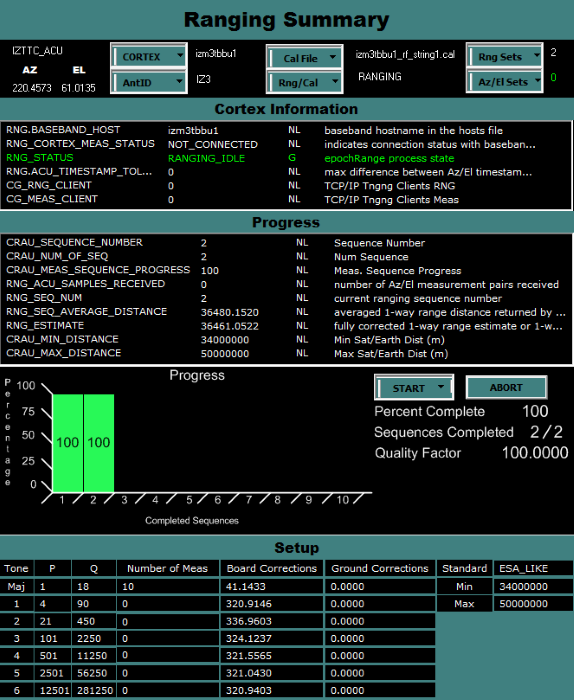
\includegraphics{./diagrams/rng_screen.png}

    Este proceso se puede monitorear desde EPOCH (Telemetry viewer y Event
viewer), podemos mencionar los siguientes puntos:

\begin{itemize}
\tightlist
\item
  El archivo de calibración de tierra se menciona en la parte superior
  de esta imagen, este debe coincidir con la configuración de RF para
  que los archivos de rango sean generados con valores correctos.
\item
  El valor de rango obtenido en la ultima secuencia de rango se
  despliega en valor de telemetría:
  \textbf{RNG\_SEQ\_AVERAGE\_DISTANCE}.
\item
  Los valores mínimos y máximos posibles se despliegan en valores de
  telemetría: \textbf{CRAU\_MIN\_DISTANCE} y
  \textbf{CRAU\_MAX\_DISTANCE}.
\item
  El progreso de la secuencia de rango se despliega como histogramas con
  hasta 10 posibles secuencias de rango por evento, este valor se
  empieza a actualizar cuando comienzan las mediciones con el tono
  mayor.
\item
  Se despliegan los valores P y Q tanto del tono mayor, como de los
  tonos menores de la secuencia de rango; estos valores son los
  necesarios para programar el cortex con nuevas frecuencias de tonos.
\item
  Se despliegan el numero de mediciones que se realizan con cada tono;
  con los tonos menores solo se elimina la ambiguedad y con el tono
  mayor se realizan las 10 mediciones de la secuencia de rango.
\item
  Se despliegan los valores de corrección de cada tono debido a la
  retransmisión por parte de la nave.
\item
  Se despliega el nombre del estándar con el que se realizan las
  mediciones: \textbf{ESA\_LIKE}.
\end{itemize}

    \begin{verbatim}
SIGNATURE:     Epoch Track File
DESCRIPTION:   Raw Range Measurement File
FILE TYPE:     TRACKING
PATH:          /home/epochtc/output/mx3/ranging/rng_data/mx3_IZ3_202002252030.trk

SPACECRAFT:    mx3
STATION:       IZ3
PHASE TYPE:    LAG
TIME UNITS:    YmdHMs3

#TONE TYPE       : ESA-Like Standard
#RANGING TYPE    : Beacon Telemetry
#GND CAL FILENAME: /home/epochtc/output/mx3/ranging/gnd_cal/izm3tbbu1_rf_string1.cal
#RANGE SEED      : 0.000000 km
#BASEBAND        : izm3tbbu1


CALIBRATION:   IZ3

2020/02/25 20:30:36.000 RANGE     0.000000 KILOMETERS
# Set ground cal to zero. Correction in range values.


TRACKING DATA:

#Corrected Tracking Data:
2020/02/25 20:30:45.134  RANGE 36461.051414 KILOMETERS
2020/02/25 20:30:45.384  RANGE 36461.051264 KILOMETERS
2020/02/25 20:30:45.634  RANGE 36461.051714 KILOMETERS
2020/02/25 20:30:45.884  RANGE 36461.051714 KILOMETERS
2020/02/25 20:30:46.134  RANGE 36461.051864 KILOMETERS
2020/02/25 20:30:46.384  RANGE 36461.052463 KILOMETERS
2020/02/25 20:30:46.634  RANGE 36461.052463 KILOMETERS
2020/02/25 20:30:46.884  RANGE 36461.052014 KILOMETERS
2020/02/25 20:30:47.134  RANGE 36461.052164 KILOMETERS
2020/02/25 20:30:47.384  RANGE 36461.051864 KILOMETERS
#Quality Factor         :        +100.000000
#Baseband Raw Time Meas :  +121684688.100000 ns,      +36480.151746 km (one-way average)
#RAW_GND_CAL            :      +63710.250701 ns,         +19.099853 km (one-way average delay subtracted from baseband raw meas)
#Fully Corrected Range  :  +121620977.849299 ns,      +36461.051894 km (one-way average)
#Baseband Timetag       : 2020/02/25 20:30:45.134 (1582662645 sec 134000 usec)

2020/02/25 20:30:57.258  RANGE 36461.051564 KILOMETERS
2020/02/25 20:30:57.508  RANGE 36461.051714 KILOMETERS
2020/02/25 20:30:57.758  RANGE 36461.052613 KILOMETERS
2020/02/25 20:30:58.008  RANGE 36461.052463 KILOMETERS
2020/02/25 20:30:58.258  RANGE 36461.052164 KILOMETERS
2020/02/25 20:30:58.508  RANGE 36461.051564 KILOMETERS
2020/02/25 20:30:58.758  RANGE 36461.052463 KILOMETERS
2020/02/25 20:30:59.008  RANGE 36461.052164 KILOMETERS
2020/02/25 20:30:59.258  RANGE 36461.052314 KILOMETERS
2020/02/25 20:30:59.508  RANGE 36461.052763 KILOMETERS
#Quality Factor         :        +100.000000
#Baseband Raw Time Meas :  +121684689.050000 ns,      +36480.152031 km (one-way average)
#RAW_GND_CAL            :      +63710.250701 ns,         +19.099853 km (one-way average delay subtracted from baseband raw meas)
#Fully Corrected Range  :  +121620978.799299 ns,      +36461.052179 km (one-way average)
#Baseband Timetag       : 2020/02/25 20:30:57.258 (1582662657 sec 258000 usec)
\end{verbatim}

    Los valores de medición quedan asentados en archivos ubicados en
izopsgs1, estos tienen un formato especifico y datos que informan al
personal de Dinámica orbital la forma en que fueron generados para
descartar incertidumbre en su calidad.

    \hypertarget{equipo-salida}{%
\subsection{Equipo (salida)}\label{equipo-salida}}

\hypertarget{configuraciuxf3n-actual}{%
\subsubsection{Configuración actual}\label{configuraciuxf3n-actual}}

    Por ultimo, solo mencionar el equipo involucrado en la secuencia de
rango.

    \begin{itemize}
\tightlist
\item
  izopsfep1
\end{itemize}

    \begin{itemize}
\tightlist
\item
  BBU1 {[}BBU2{]}
\end{itemize}

    \begin{itemize}
\tightlist
\item
  UC1 {[}UCR{]}
\end{itemize}

    \begin{itemize}
\tightlist
\item
  HPA1 {[}HPAR{]}
\end{itemize}

    \begin{itemize}
\tightlist
\item
  Antenna Feeder
\end{itemize}

    \hypertarget{equipo-entrada}{%
\subsection{Equipo (entrada)}\label{equipo-entrada}}

\hypertarget{configuraciuxf3n-actual}{%
\subsubsection{Configuración actual}\label{configuraciuxf3n-actual}}

    Y de salida.

    \begin{itemize}
\tightlist
\item
  Antenna Feeder
\end{itemize}

    \begin{itemize}
\tightlist
\item
  {[}LNA1{]} LNA2 {[}LNA3{]}
\end{itemize}

    \begin{itemize}
\tightlist
\item
  DC1
\item
  DCR
\end{itemize}

    \begin{itemize}
\tightlist
\item
  BBU1
\item
  BBU2
\end{itemize}

    \hypertarget{en-conclusiuxf3n}{%
\subsubsection{En conclusión}\label{en-conclusiuxf3n}}

    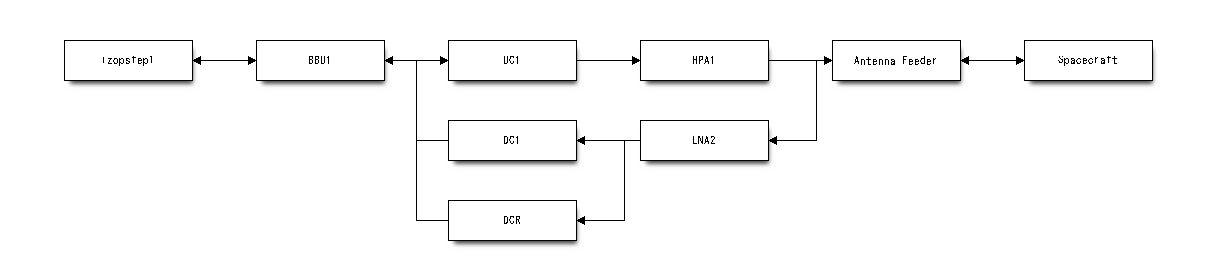
\includegraphics{./diagrams/diagrama_mx3.png}

    \hypertarget{gracias-por-su-tiempo}{%
\section{Gracias por su tiempo}\label{gracias-por-su-tiempo}}


    % Add a bibliography block to the postdoc



\end{document}
